%=====================================================================================================
% Document formatting and packages
%=====================================================================================================

\documentclass[10pt]{article}
\setlength\topmargin{0in}
\setlength\headheight{0in}
\setlength\headsep{0in}
\setlength\textheight{9in}
\setlength\textwidth{6.5in}
\setlength\oddsidemargin{0in}
\setlength\evensidemargin{0in}
\setlength\parindent{0.25in}
\setlength\parskip{0in} 

\usepackage{amsmath}
\usepackage{bm}													% required for bold equations
\usepackage{graphicx}										% required for images
\usepackage{epstopdf}										% require for .eps graphics
\usepackage{float}											% allows [H] to be used for floats (forces float to appear at location in code) 
\usepackage[usenames,dvipsnames]{color}
\usepackage[pdftex]{hyperref} 					% creates bookmarks and all cross-references and citations are hyperlinked in pdf
\hypersetup{bookmarksnumbered, 					% put section numbers in bookmarks
						bookmarksopen=false,
						colorlinks = true,
						linkcolor=CadetBlue,
						citecolor=CadetBlue,
						urlcolor=MidnightBlue}			% bookmarks expanded when pdf opened	
						
\usepackage{C:/MyFiles/Reference_Libraries/LaTeX/MiscPackages/fixfoot/fixfoot}
						
						
%=====================================================================================================
% My Macros
%=====================================================================================================								

\DeclareFixedFootnote{\gyrofootnote}{x-IMUs of generations prior to version 1.3 use the \href{http://www.x-io.co.uk/res/doc/itg3200.pdf}{ITG-3200} gyroscope.}
				
\def \xIMUGUI {\href{http://www.x-io.co.uk/node/9\#ximugui}{x-IMU GUI}}
\def \xIMUAPI {\href{http://www.x-io.co.uk/node/9\#ximuapi}{x-IMU API}}		
\def \MATLAB {\href{http://www.x-io.co.uk/node/10\#matlab_import_ximu_data}{MATLAB}}					
\def \accelMagName {\href{http://www.x-io.co.uk/res/doc/lsm303dlh.pdf}{LSM303DLH}}
\def \gyroName {\href{http://www.x-io.co.uk/res/doc/imu3000.pdf}{IMU-3000}\gyrofootnote{}}	

\def \contactUs {\href{http://www.x-io.co.uk/contact}{contact us}}
\def \sectionComingSoon {This section is currently unavailable but can be updated \href{http://www.x-io.co.uk/contact}{on request}.}				
						
%=====================================================================================================
% Title, Name, Date
%=====================================================================================================

\title{\Huge x-IMU User Manual 1.0 \normalsize}
\author{x-io Technologies}

\begin{document}

%---------------------------------------------------------------------------------------------------
\begin{titlepage}

	\maketitle
	\vspace{20 mm}
	\begin{figure}[H]
		\centering
			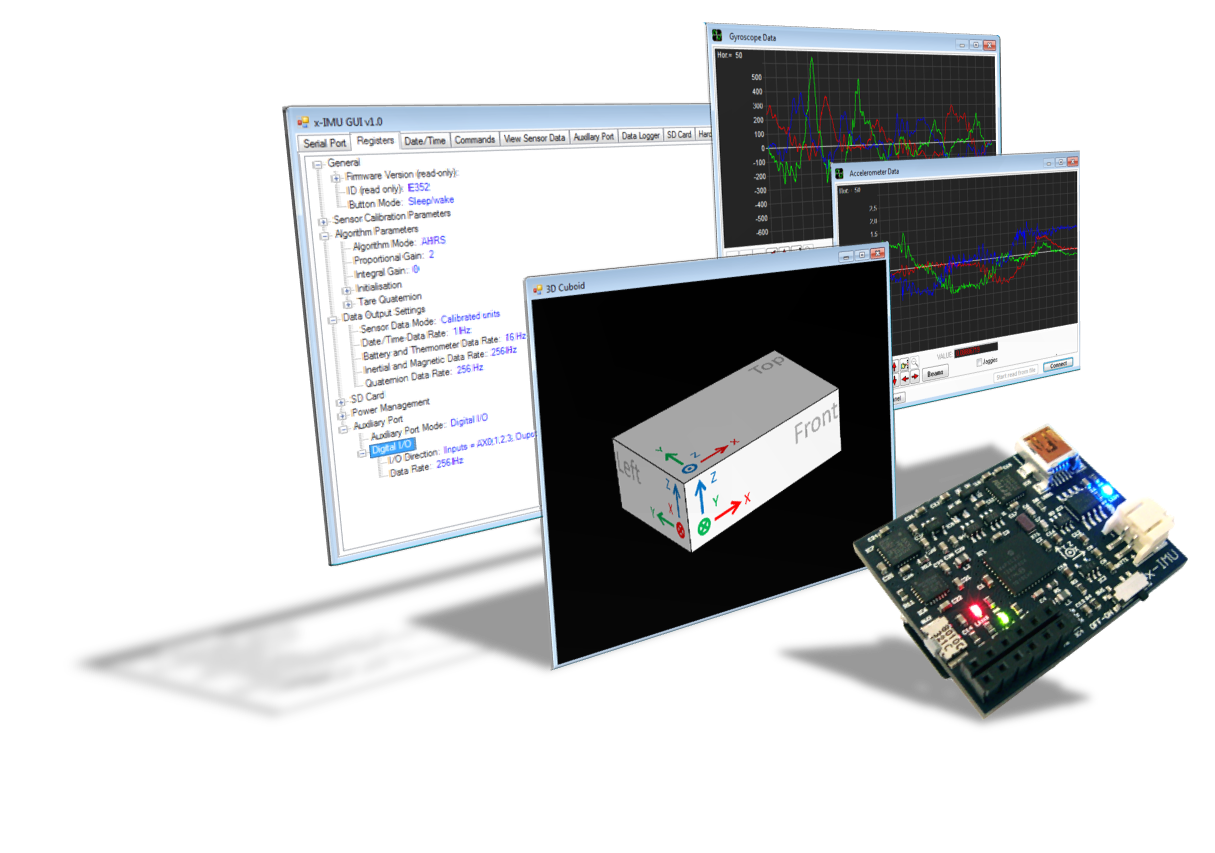
\includegraphics[width=0.8\textwidth]{graphics/ximu_software_large.png}
	\end{figure}

\end{titlepage}

%=====================================================================================================
% Version history
%=====================================================================================================
%\section{Version history}
%\label{sec:VersionHistory}

\begin{table}[H]
	\centering
		\begin{tabular*}{1.0\textwidth}{l l p{0.7\textwidth}}
			\hline
			Version	&	Date				& Notes							\\
			\hline																		\\
			1.0			& 10/05/2011	&	Initial release.  Compatible versions: Firmware 4.x, GUI 6.x, API 7.x.  \\
			\hline
		\end{tabular*}
		\caption{Version history}
\end{table}

%If you have any suggestions for how this document could be improved, please \href{ http://www.x-io.co.uk/contact}{contact us} and let us know.

\newpage
%=====================================================================================================
% Disclaimer
%=====================================================================================================
\section*{Disclaimer}
\label{sec:Disclaimer}

%The x-IMU was devleoped to be an accessable and affordable research tool.  x-io Technolgoies does not provide any guarentees of performance

The x-IMU and associated software are provided in an `as in' condition.  No warranties, whether express, implied or statutory, including but not limited to implied warranties of merchantability and fitness for a particular purpose apply.  x-io Technologies shall not in any circumstances, be liable for special, incidental or consequential damages, for any reason whatsoever.

\newpage
%=====================================================================================================
% Table of contents
%=====================================================================================================

\tableofcontents

\newpage
%=====================================================================================================
% x-IMU overview
%=====================================================================================================
\section{x-IMU overview}
\label{sec:xIMUOverview}

The x-IMU was designed to be the most versatile IMU/AHRS product available. Its host of on-board sensors, algorithms and configurable 8-channel auxiliary port make the x-IMU both a powerful sensor and controller. Communication is enabled via USB or Bluetooth for wireless applications. The on-board SD card, battery charger (via USB), real-time clock/calendar and motion trigger wake up also make the x-IMU an ideal stand-alone data logger.

The open source \xIMUGUI{} allow users configure all internal x-IMU settings, view sensor data in real-time and export data to software such as \MATLAB{} and Microsoft Excel. Custom user software may be developed using the \xIMUAPI{}.

\subsection{x-IMU Features}
\label{sec:xIMUFeatures}

\paragraph{On-board sensors}
\begin{itemize}
	\item Triple axis 16-bit gyroscope (�2000 $^\circ$/s range)
	\item Triple axis 12-bit accelerometer (Configurable range up to �8 g)
	\item Triple axis 12-bit magnetometer (Configurable range up to �8.1 G)
	\item 16-bit thermometer
	\item Battery level
	\item Calibrated and temperature compensated (gyroscope only)
	\item Configurable sample rates up to 256 Hz
\end{itemize}

\paragraph{On-board algorithms}
\begin{itemize}
    \item IMU algorithm for real-time measurement of pitch and roll relative to the Earth surface, immune to magnetic inferences
    \item AHRS algorithm for real-time measurement of full orientation relative to the Earth coordinate frame
    \item Sensor calibration algorithms for user maintenance
\end{itemize}    

\paragraph{Connectivity}
\begin{itemize}
    \item USB
    \item Bluetooth (Class 1, 100m range, SPP)
    \item Micro-SD card (Supports SDHC and FAT16/32 for capacities up to 2 TBs)
\end{itemize}    

\paragraph{Power options}
\begin{itemize}
    \item USB
    \item LiPo battery (On-board charging via USB)
    \item External source (3.6 V to 7.7 V)
    \item Low power consumption (35 mA to 100 mA dependant on settings and usage, 130 �A sleep mode)
\end{itemize}    

\paragraph{Low profile}
\begin{itemize}
    \item Dimensions: 33 $\times$ 42 $\times$ 10 mm
    \item Weight: 12g
\end{itemize}  

\paragraph{Other features}
\begin{itemize}
    \item Motion triggered wake-up and sleep
    \item Real-time clock and calendar
    \item Configurable command button
    \item Configurable 8 channel auxiliary port
\end{itemize}    

\paragraph{Auxiliary port modes}
\begin{itemize}
    \item Digital I/O (Outputs controlled via USB or Bluetooth)
\end{itemize}    

\subsection{x-IMU Software}
\label{sec:xIMUSoftware}

The \xIMUGUI{} (Graphical User Interface) provides interface to all features and functionality of the x-IMU via the \xIMUAPI{}. The \xIMUGUI{} is open source and is intended to serve as a comprehensive template for those using the \xIMUAPI{} to develop their own applications. Additional software examples using the \xIMUAPI{} for different applications can be found on the \href{http://www.x-io.co.uk/node/10}{x-IMU Examples webpage}.

\paragraph{Features}
\begin{itemize}
    \item View, edit and backup all internal x-IMU settings
    \item Real-time 2D and 3D data graphics
    \item Control panels for auxiliary port
    \item Data logger and file converter for exporting data; e.g. to MATLAB, Microsoft Excel, etc.
    \item Magnetic calibration tools
    \item Firmware bootloader to access new features in future x-IMU firmware versions
\end{itemize}    


\newpage
%=====================================================================================================
% Getting started
%=====================================================================================================
\section{Getting started}
\label{sec:GettingStarted}

\begin{enumerate}
	\item Install the USB drivers (\ref{sec:InstallingUSBDrivers}) and/or pair the x-IMU as a Bluetooth device (\ref{sec:PairingTheXIMUWithABluetoothHost}).
	\item Download and install the latest version of the \xIMUGUI{}.
	\item Connect to the x-IMU via the \textit{Serial port} tab page (\ref{sec:TabPageSerialPort}) of the \xIMUGUI{}.
\end{enumerate}

The x-IMU and accompanying software were designed to be versatile and intuitive.  New users are advised to explore the x-IMU through the \xIMUGUI{} and consult this user manual when required.  If you are struggling to use the system and feel that this user manual is not providing you with appropriate documentation, please \contactUs{} so that we update the document appropriatly.



%\subsection{Step 1 - Install Software and drivers}
%\label{sec:Step1InstallSoftwareAndDrivers}
%
%download latest version of \xIMUGUI{}
%
%\subsection{Step 2 - Connect to serial port (via USB or Bluetooth)}
%\label{sec:Step2ConnectToSerialPortViaUSBOrBluetooth}
%
%\subsection{Step 3 - Configure and use device}
%\label{sec:Step3ConfigureAndUseDevice}


\newpage
%=====================================================================================================
% Hardware overview
%=====================================================================================================
\section{Hardware overview}
\label{sec:HardwareOverview}

\begin{figure}[H]
	\centering
		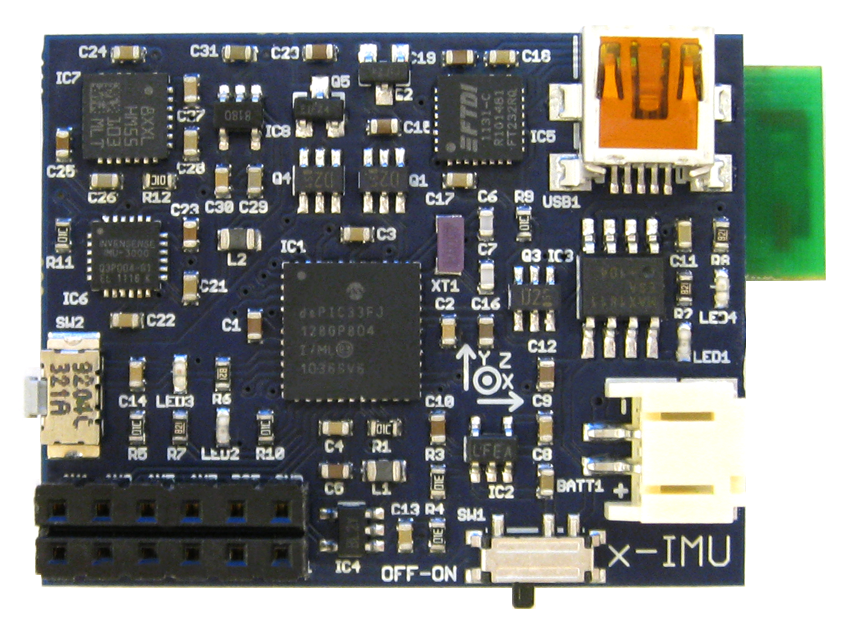
\includegraphics[width=0.5\textwidth]{graphics/ximu_pcb_top_large.png}
		\caption{x-IMU top}
	\label{fig:ximu_pcb_top_large}
\end{figure}

\begin{figure}[H]
	\centering
		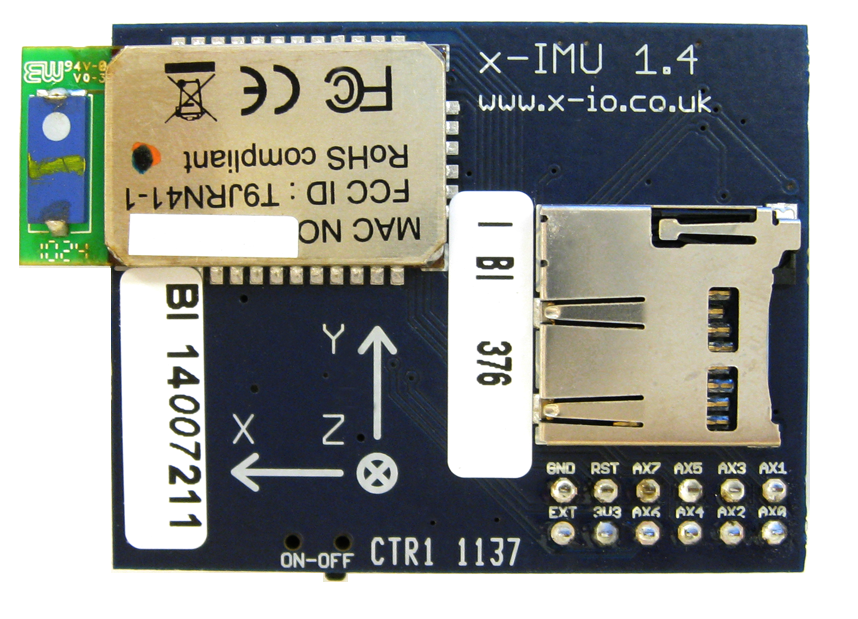
\includegraphics[width=0.5\textwidth]{graphics/ximu_pcb_bottom_large.png}
		\caption{x-IMU bottom}
	\label{fig:ximu_pcb_bottom_large}
\end{figure}

%---------------------------------------------------------------------------------------------------
\subsection{Power switch}
\label{sec:PowerSwitch}

The power switch is used to switch the battery and USB power on or off.  The battery and USB power is completely disconnected when the switch is in the \textit{off} position.  The x-IMU may be powered by an external supply (\ref{sec:ExternalSupply}) via the auxiliary port (\ref{sec:AuxiliaryPort}).  For this the power switch must be in the \textit{off} position.

%The on-board USB (\ref{sec:USB}) and battery charging (\ref{sec:BatteryAndCharging}) are powered directly from the computer USB port so the x-IMU does not need to be switched on to be recognised by the computer or to charge the battery.  The on-board real-time clock and calendar (\ref{sec:RealTimeClockAndCalendar}) will only be maintained while the x-IMU is powered.  Applications that require date and time to be maintained should ensure that the x-IMU is never switched off and instead take advantage of sleep mode (\ref{sec:SleepMode}).

%---------------------------------------------------------------------------------------------------
\subsection{Push button}
\label{sec:PushButton}

The push button may be configured to execute x-IMU commands (\ref{sec:Commands}).  The mode of the push button is defined in the \textit{Button mode} register (\ref{sec:ButtonMode}).  The default mode is \textit{sleep/wake}.

%---------------------------------------------------------------------------------------------------
\subsection{LEDs}
\label{sec:LEDs}

%------------------------------------------------
\subsubsection{Status LED (Green)}
\label{sec:StatusLEDGreen}

The green LED indicates the status of the x-IMU.  The green LED will remain lit while the device is sampling and sending data packets and will otherwise be extinguished; for example, during the execution of commands (\ref{sec:Commands}).  In sleep mode (\ref{sec:SleepMode}) the green LED will blink once every 3 seconds.  The green LED will flash rapidly while the on-board bootloader is active.

%------------------------------------------------
\subsubsection{SD card LED (Amber)}
\label{sec:SDCardLEDAmber}

The amber LED indicates SD card (\ref{sec:SDCard}) activity.  Details on the SD LED behaviour are provided in the SD card LED section (\ref{sec:SDCardLED}).

%------------------------------------------------
\subsubsection{Bluetooth LED (Blue)}
\label{sec:BluetoothLEDBlue}

The blue LED indicates the state of the Bluetooth (\ref{sec:Bluetooth}) connection and power status.  Details of the Bluetooth LED behaviour are summarised in Table \ref{tab:BluetoothLEDstates}.

%------------------------------------------------
\subsubsection{Charging LED (Red)}
\label{sec:ChargingLEDRed}

The red LED indicates the charging state of the battery (\ref{sec:BatteryAndCharging}).  The red LED will remain lit while the battery is charging and will be extinguished once the battery is charged.

%---------------------------------------------------------------------------------------------------
\subsection{USB socket}
\label{sec:USBSocket}

The USB mini-B socket is used to connect the x-IMU to a computer via a standard USB \textit{A to mini B (5 pin)} type cable.  The USB connect can also be used to power the x-IMU.  See the USB section (\ref{sec:USB}) for more information.

%---------------------------------------------------------------------------------------------------
\subsection{micro-SD card socket}
\label{sec:microSDCardSocket}

The micro SD card socket is used to log all data generated by the x-IMU to an SD card.  The x-IMU supports standard SD and HCSD cards formatted as either FAT16 or FAT32.  A new file is created and logging starts each time the x-IMU is switch on, wakes up or is reset.  The file is automatically closed when the x-IMU enters sleep mode (\ref{sec:SleepMode}) or is reset.  The file must be closed before the SD card is removed or the x-IMU switched of otherwise the current file will corrupt and data lost.  See the SD card section (\ref{sec:SDCard}) for more information.

%---------------------------------------------------------------------------------------------------
\subsection{Bluetooth radio}
\label{sec:BluetoothRadio}

The on-board Bluetooth radio is used to connect the x-IMU to a computer via Bluetooth.  The on-board Bluetooth radio is a class I device with a maximum range of 100 m.  The radio uses the Serial Port Profile (SPP) to enable connection to any Bluetooth host without the need to install specific drivers.  Power to the Bluetooth radio can be disabled (\ref{sec:BluetoothPower}) to converse power.  See the Bluetooth section (\ref{sec:BluetoothRadio}) for more information.

%---------------------------------------------------------------------------------------------------
\subsection{Battery connector}
\label{sec:BatteryConnector}

The on-board battery connector allows the x-IMU to be powered by any single-cell Lithium Polymer battery.  The battery is automatically charged while the x-IMU is connected via USB.  See the battery and charging section (\ref{sec:BatteryAndCharging}) for more information.

%%---------------------------------------------------------------------------------------------------
%\subsection{Auxiliary port}
%\label{sec:subAuxiliaryPort}
%
%The auxiliary port can be configured to
%
%...consists of 8 channels, power in, $3.3 V$ out, external power supply in, hard reset


\newpage
%=====================================================================================================
% Software overview
%=====================================================================================================
\section{Software overview}
\label{sec:SoftwareOverview}

%The x-IMU software consists of the \xIMUGUI{} and \xIMUAPI{}.  
%
%%---------------------------------------------------------------------------------------------------
%\subsection{Installing software and drivers}
%\label{sec:InstallingSoftwareAndDrivers}
%
%...
%
%%------------------------------------------------
%\subsubsection{Uninstalling software}
%\label{sec:UninstallingSoftware}
%
%May first need to uninstiall x-IMU GUI before installing newer version.

%---------------------------------------------------------------------------------------------------
\subsection{x-IMU GUI}
\label{sec:xIMUGUI}

%...

%------------------------------------------------
\subsubsection{Tab page: Serial port}
\label{sec:TabPageSerialPort}

The serial port tab page is used to manage the USB or Bluetooth connection between the software and the x-IMU.  The USB and Bluetooth connections will each appear as a separate serial port; see the USB section (\ref{sec:USB}) and Bluetooth section (\ref{sec:Bluetooth}) for more information and how to find the serial port name assigned to each connection.

To connect to the x-IMU, the user first select the correct serial port name the x-IMU appears as in the \textit{Port name} drop down list.  If the name does not appear in the list, the user can either press the \textit{Refresh List} button to update the drop down list or type in the port name directly.  The \textit{Open Port} button may then be pressed to connect to the device.

\begin{figure}[H]
	\centering
		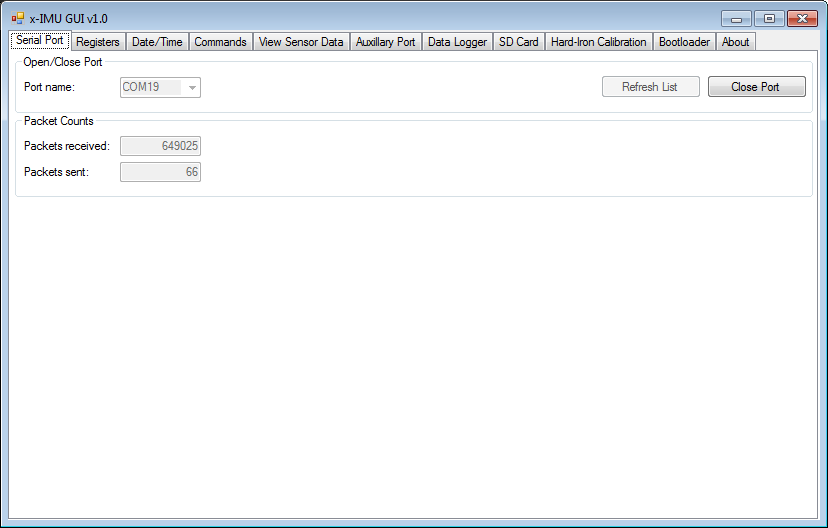
\includegraphics[width=0.8\textwidth]{graphics/GUI_tab_serial_port.png}
		\caption{\xIMUGUI{} serial port tab page}
	\label{fig:GUI_tab_serial_port}
\end{figure}

%------------------------------------------------
\subsubsection{Tab page: Registers}
\label{sec:TabPageRegisters}

The registers tab page allows the user to view, edit and back up all internal settings on the x-IMU; see the registers section (\ref{sec:Registers}) for more infomation on x-IMU registers.  All registers are organised into sections within a tree view where the end node of each branch is an individual register name and text box or drop down list containing the register value.  Register values that have been read directly from the x-IMU or loaded from file will appear as blue text.  Any registers values then edited will appear as red text.  A right click on any register will show the action menu.

To read all register on the x-IMU, the user should right click anywhere in the registers tab page and select \textit{Read all registers}.  The software will then read each register and update the values in the tree view.  Individual registers or groups of registers may be read by first selecting a register or group within the tree view and then selecting \textit{Read this register only} or \textit{Read all registers in this group only}.  Register values in the tree view may be written to teh x-IMU using the \textit{Write all regisers}, \textit{Write this register only} and \textit{Write all registers in this group only} options in the action menu.

\begin{figure}[H]
	\centering
		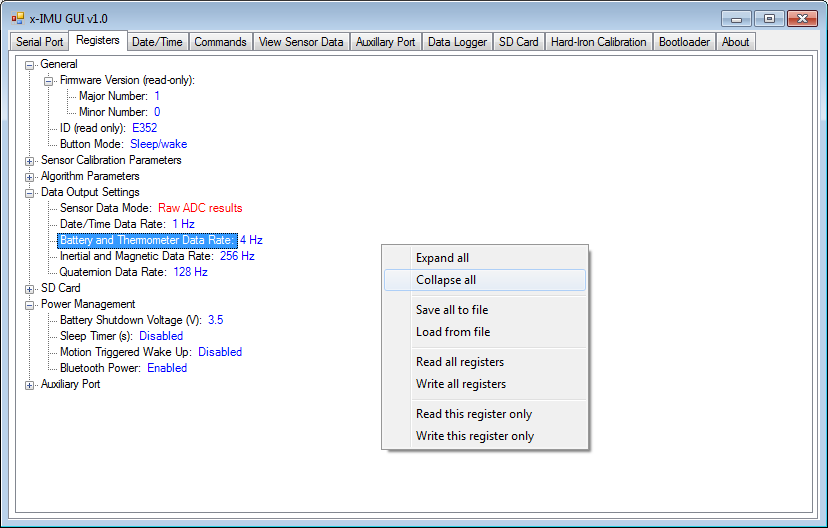
\includegraphics[width=0.8\textwidth]{graphics/GUI_tab_registers.png}
		\caption{\xIMUGUI{} registers tab page with (right click) action menu}
	\label{fig:GUI_tab_registers}
\end{figure}

%------------------------------------------------
\subsubsection{Tab page: Date/time}
\label{sec:TabPageDateTime}

The date/time tab page allows the user to view and set the date and time of the x-IMU's real-time clock and calendar.  The \textit{Received date/time} text box displays the date and time each time it is received from the x-IMU.  The \textit{Read Date/Time} button may be used to read the current date and time of the x-IMU; this is of use if date/time data rate has been disabled.  Pressing the \textit{Set Date/Time} button will set the x-IMU date and time equal to computer date and time.

\begin{figure}[H]
	\centering
		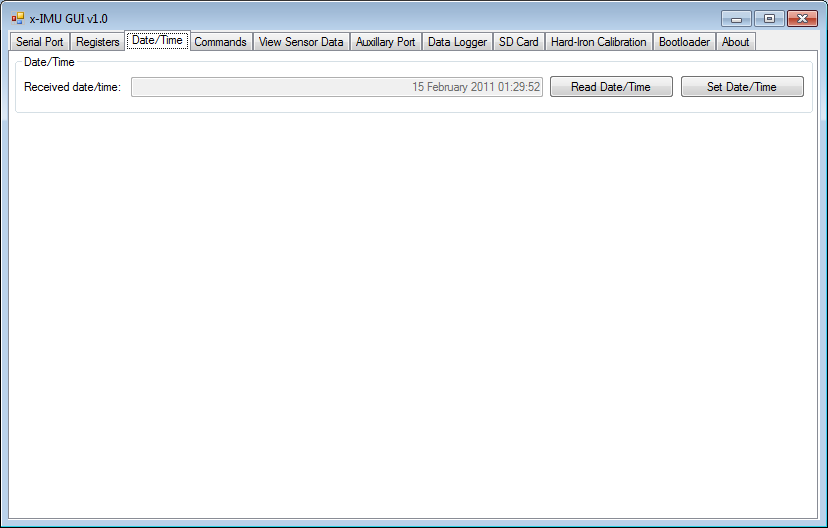
\includegraphics[width=0.8\textwidth]{graphics/GUI_tab_date_time.png}
		\caption{\xIMUGUI{} date/time tab page}
	\label{fig:GUI_tab_date_time}
\end{figure}

%------------------------------------------------
\subsubsection{Tab page: Commands}
\label{sec:TabPageCommands}

The commands tab page is used to send commands to the x-IMU.  See the commands section (\ref{sec:Commands}) for more information on individual commands.  Once the x-IMU has processed a command it will echo the command back and it will appear in a message box.  To suppress these message boxes, un-check the \textit{Display received command messages in message box} check box.

\begin{figure}[H]
	\centering
		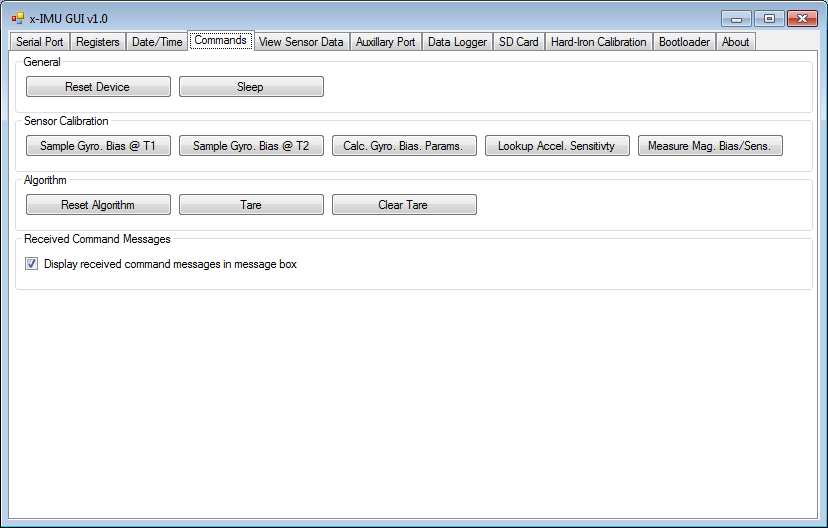
\includegraphics[width=0.8\textwidth]{graphics/GUI_tab_commands.png}
		\caption{\xIMUGUI{} date/time tab page}
	\label{fig:GUI_tab_commands}
\end{figure}

%------------------------------------------------
\subsubsection{Tab page: View sensor data}
\label{sec:TabPageViewSensorData}

The view sensor data tab page contains buttons to show or hide separate real-time data graphic windows for incoming x-IMU sensor data.

\begin{figure}[H]
	\centering
		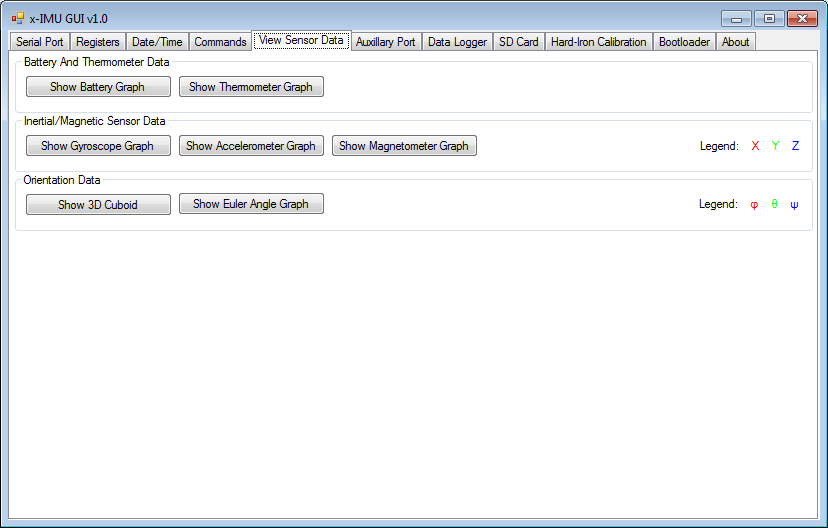
\includegraphics[width=0.8\textwidth]{graphics/GUI_tab_view_sensor_data.png}
		\caption{\xIMUGUI{} view sensor data tab page}
	\label{fig:GUI_tab_view_sensor_data}
\end{figure}

The data from individual sensors is displayed in real-time data graphs as seen in Figure \ref{fig:GUI_tab_view_sensor_data}.  The controls bar at the bottom of each graph allow the view and scaling to be adjusted.
  
\begin{figure}[H]
	\centering
		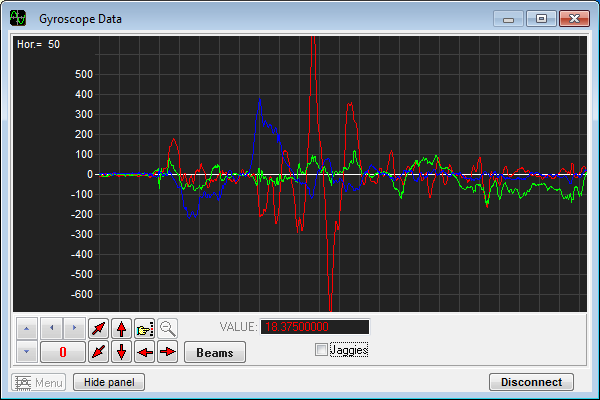
\includegraphics[width=0.5\textwidth]{graphics/GUI_gyroscope_graph.png}
		\caption{\xIMUGUI{} gyroscope data window}
	\label{fig:GUI_gyroscope_graph}
\end{figure}

Orientation data received may be displayed in a graph as ZYX Euler angles and displayed as the orientation of a 3D cuboid as seen in figure \ref{fig:GUI_3D_cuboid}.  The cuboid is displayed in a screen coordinate frame where the x-axis is aligned to the width of the screen (left to right), the z-axis aligned to the height (bottom to top) and the y-axis projects into the screen.  To align the motion of the physical x-IMU and 3D cuboid displayed on the screen, the user should first align the axes of the physical x-IMU to the screen coordinate frame and then use the \textit{Tare} command (\ref{sec:Tare}).

\begin{figure}[H]
	\centering
		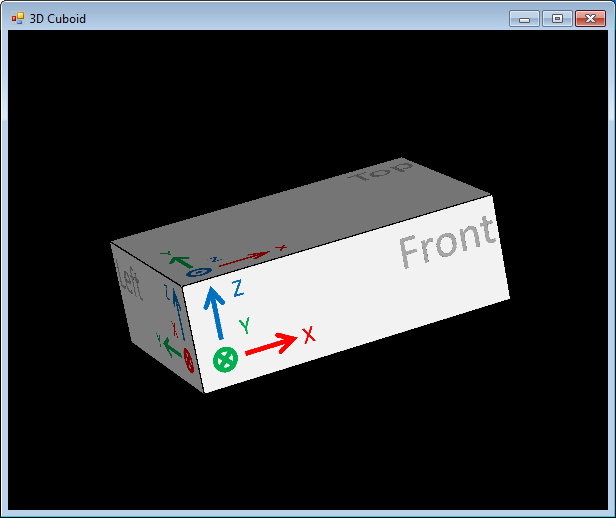
\includegraphics[width=0.5\textwidth]{graphics/GUI_3D_cuboid.png}
		\caption{\xIMUGUI{} 3D cuboid window}
	\label{fig:GUI_3D_cuboid}
\end{figure}

%------------------------------------------------
\subsubsection{Tab page:  Auxillary port}
\label{sec:TabPageAuxillaryPort}

The auxiliary port tab page contains buttons to show or hide individual control windows for the different modes of the auxiliary port.

\begin{figure}[H]
	\centering
		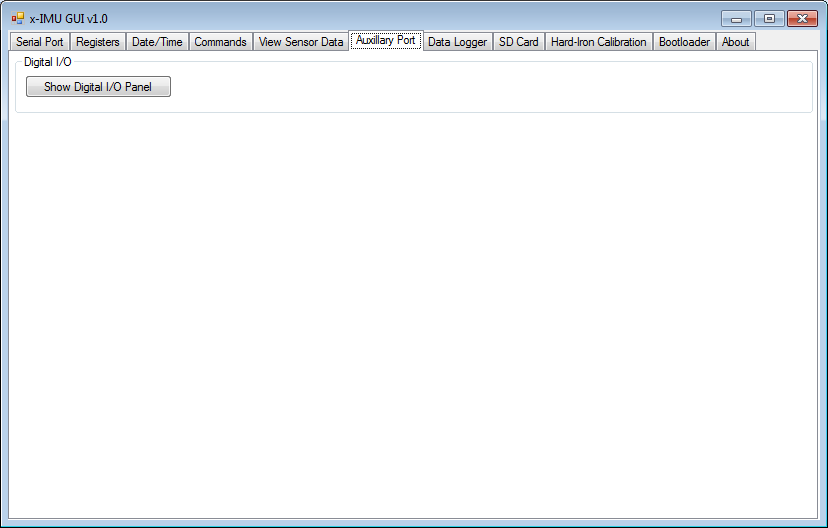
\includegraphics[width=0.8\textwidth]{graphics/GUI_tab_auxiliary_port.png}
		\caption{\xIMUGUI{} auxiliary port tab page}
	\label{fig:GUI_tab_auxiliary_port}
\end{figure}

\paragraph{Digital I/O control panel}
\label{sec:DigitalIOControlPanel}
The digital I/O control panel displays the state and mode of each channel of the auxiliary port when in digital I/O mode as shown in figure \ref{fig:GUI_digital_IO_control_panel}.  Each channel is represented by a check box.  If the channel mode is output then the check box is enabled and may be checked or un-checked to set the channel high or low respectively.  If the channel is an input the check box is disabled and will be checked or un-checked if the channel is high or low respectively.

\begin{figure}[H]
	\centering
		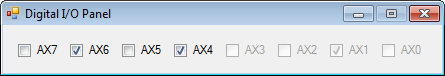
\includegraphics[width=0.4\textwidth]{graphics/GUI_digital_IO_control_panel.png}
		\caption{\xIMUGUI{} digital I/O control panel}
	\label{fig:GUI_digital_IO_control_panel}
\end{figure}

%------------------------------------------------
\subsubsection{Tab page:  Data logger}
\label{sec:TabPageDataLogger}

The data logger tab allows the user to log incoming real-time data to file.  These files may be imported to user software such as Microsoft Excel and MATLAB.  The user may select the location and first part of the file name in the \textit{File path} text box.  This file name will be extended with an appropriate description and extension when the individual data files are created.  For example, if a file name of \verb=myFile= is specified, Euler angle and date/time data will be saved to \verb=myFile_EulerAngles.csv= and \verb=myFile_DateTime.txt=.

\begin{figure}[H]
	\centering
		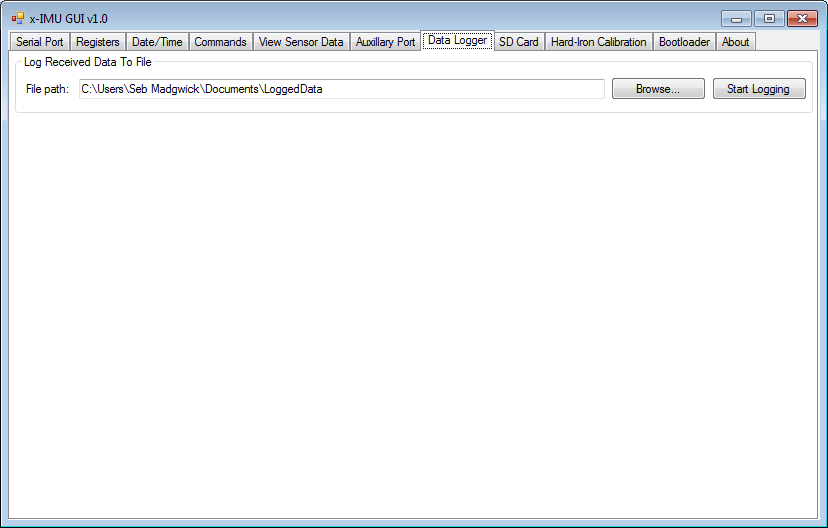
\includegraphics[width=0.8\textwidth]{graphics/GUI_tab_data_logger.png}
		\caption{\xIMUGUI{} data logger tab page}
	\label{fig:GUI_tab_data_logger}
\end{figure}

The \textit{Start/Stop Logging} button is used to start and stop the data logger.  When logging is stopped, a report window will be presented detailing the number of each type of packet logged and the specific data files created; as shown in figure \ref{fig:GUI_data_logger_report}.

\begin{figure}[H]
	\centering
		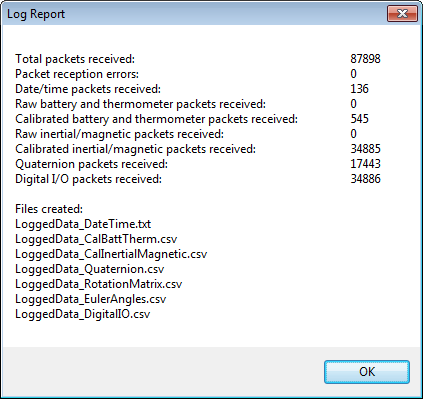
\includegraphics[width=0.4\textwidth]{graphics/GUI_data_logger_report.png}
		\caption{\xIMUGUI{} data logger report}
	\label{fig:GUI_data_logger_report}
\end{figure}

%------------------------------------------------
\subsubsection{Tab page:  SD card}
\label{sec:TabPageSDCard}

The SD card tab page allows the user to convert binary files (\verb=.bin=) saved to the SD card in to readable data files.  These files may be imported to user software such as Microsoft Excel and MATLAB.  The location and file name must be specified in the \textit{File path} text box.  The file conversion will start when the \textit{Convert} button is clicked.  This process occurs in the background and may take a while if a large binary file is specified.

\begin{figure}[H]
	\centering
		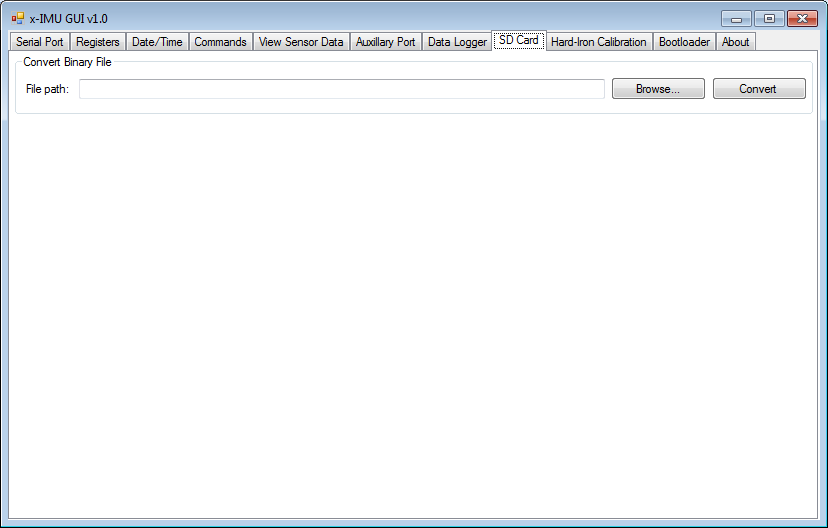
\includegraphics[width=0.8\textwidth]{graphics/GUI_tab_SD_card.png}
		\caption{\xIMUGUI{} SD card tab page}
	\label{fig:GUI_tab_SD_card}
\end{figure}

Once the conversion is complete, a report window will be presented detailing the number of each type of packet read and the specific data files created; as shown in figure \ref{fig:GUI_conversion_report}.

\begin{figure}[H]
	\centering
		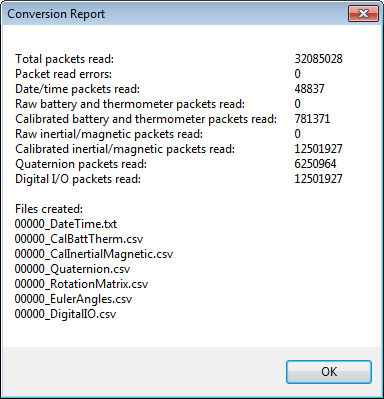
\includegraphics[width=0.35\textwidth]{graphics/GUI_conversion_report.png}
		\caption{\xIMUGUI{} binary file conversion report}
	\label{fig:GUI_conversion_report}
\end{figure}

%------------------------------------------------
\subsubsection{Tab page:  Hard-iron calibration}
\label{sec:TabPageHardIronCalibration}

The hard-iron calibration tab page provides all the functionality required for the user to calibrate for hard-iron interferences affecting the x-IMU.  It is necessary to re-calibrate hard-iron parameters whenever the x-IMU's magnetic characterises are changed; for example, when the x-IMU if fitted to a battery or mounting that includes ferromagnetic elements.  The 3 group boxes, \textit{Step 1 - Clear Hard-Iron Bias Registers}, \textit{Step 2 - Collect Hard-Iron Calibration Dataset} and \textit{Step 3 - Run Hard-Iron Calibration Algorithm} represent the 3 steps that must be performed in order.  See the hard-iron calibration section (\ref{sec:HardIronCalibration}) for more information.

\begin{figure}[H]
	\centering
		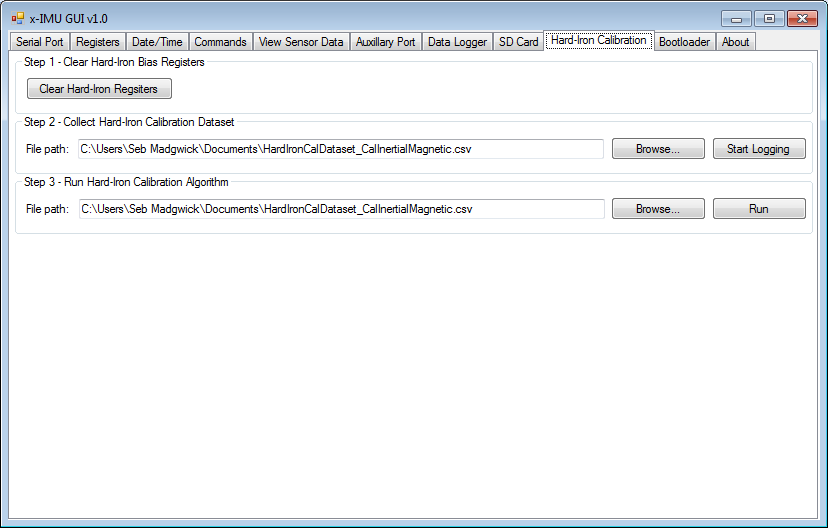
\includegraphics[width=0.8\textwidth]{graphics/GUI_tab_hard_iron_calibration.png}
		\caption{\xIMUGUI{} hard-iron calibration tab page}
	\label{fig:GUI_tab_hard_iron_calibration}
\end{figure}

%------------------------------------------------
\subsubsection{Tab page:  Bootloader}
\label{sec:TabPageBootloader}

The bootloader tab page allows the x-IMU firmware to be updated.  The bootloader may only be used while the x-IMU is connected via USB and the serial port closed.  See the bootloader section (\ref{sec:Bootloader}) for more information.

%\begin{figure}[H]
%	\centering
%		\includegraphics[width=0.8\textwidth]{graphics/GUI_tab_bootloader.png}
%		\caption{\xIMUGUI{} bootloader tab page}
%	\label{fig:GUI_tab_bootloader}
%\end{figure}

%---------------------------------------------------------------------------------------------------
\subsection{x-IMU API}
\label{sec:xIMUAPI}

The \xIMUAPI{} (Application Programming Interface) is a code library that contains all the classes, data structures and methods required to interface to all features and functionality of the x-IMU.  The \xIMUAPI{} is an open source project written in C\# and targets Microsoft .NET 3.5.  Documentation for use of the API is represented by the XML comments throughout the source code which is accessed automatically by Visual Studio's Intellisense.  The open source \xIMUGUI{} serves as a comprehensive template for use of all features of the \xIMUAPI{}.  Further examples for specific applications are provided on the \href{http://www.x-io.co.uk/node/10}{x-IMU Examples} web page.

\newpage
%=====================================================================================================
% USB
%=====================================================================================================
\section{USB}
\label{sec:USB}

The x-IMU streams all communication data simultaneously and identically via USB, Bluetooth (\ref{sec:Bluetooth}) and to a file on the SD card (\ref{sec:SDCard}).  The USB and Bluetooth connections are also be used to send commands (\ref{sec:Commands}), read/write registers and settings (\ref{sec:Registers}) and control the auxiliary port outputs (\ref{sec:AuxiliaryPort}) from the host computer.  As both USB and Bluetooth connections appear as serial ports, use of either communication channel is identical.

The x-IMU can be connected to a computer via a standard USB \textit{A to mini B (5 pin)} type cable.  The on-board FTDI USB chip is widely used USB interface with \href{http://www.ftdichip.com/Drivers/VCP.htm}{drivers available} for Windows, Mac OS X and Linux.  Once the drivers have been installed (\ref{sec:InstallingUSBDrivers}) and the x-IMU connected to the computer, the x-IMU will appear as a serial port and be assigned an available port name; for example \textit{COM2}.  The computer may then communicate with the x-IMU by opening this serial port.  This is achieved via the \textit{Serial Port} tab page (\ref{sec:TabPageSerialPort}) of the \xIMUGUI{}.

The USB connection is a reliable communication channel that cannot be comprised by user settings; the x-IMU will not enter \textit{sleep mode} (\ref{sec:SleepMode}) due to the \textit{sleep timer} (\ref{sec:SleepTimer}) or \textit{low battery voltage detection} (\ref{sec:LowBatteryVoltageDetection}) while the USB is connected.  The USB connection can be used to power the x-IMU and is used by the on-board charging circuit to charge the battery if attached (\ref{sec:BatteryAndCharging}).  The on-board USB interface is powered directly by the USB connection, this means that the x-IMU will remain detectable and the serial port held open by the computer even while the x-IMU is switched off or in sleep mode (\ref{sec:SleepMode}).

%---------------------------------------------------------------------------------------------------
\subsection{Installing USB drivers}
\label{sec:InstallingUSBDrivers}

The Windows USB drivers can be downloaded from the \href{http://www.x-io.co.uk/node/9}{x-IMU webpage}.  Drivers for other operating systems are available of the \href{http://www.ftdichip.com/Drivers/VCP.htm}{FTDI website}.  To install the Windows drivers, simply run the \verb=.exe= file.  This will automatically detect specific Windows operating system being used and install the correct drivers.  Once the drivers have been installed and the x-IMU connected to the computer, the x-IMU will appear as a serial port and be assigned an available port name; for example \textit{COM2}.  The port name assigned to the x-IMU USB connection can be confirmed at any time by viewing the computer's \textit{Ports} in Windows device manager; as shown in Figure \ref{fig:BluetoothServices}.

\begin{figure}[H]
	\centering
		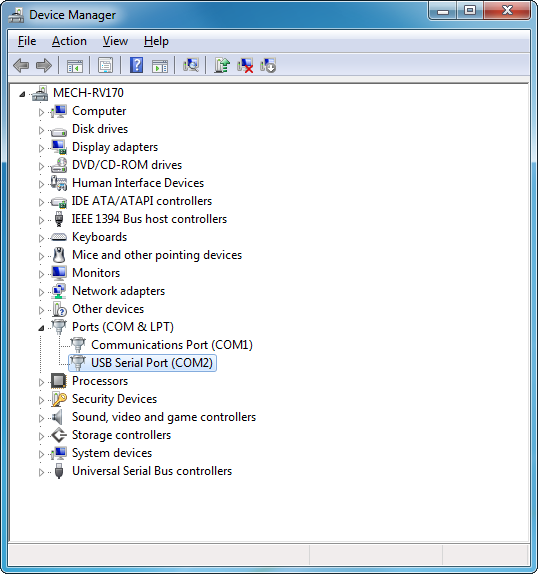
\includegraphics[width=0.5\textwidth]{graphics/USBportName.png}
		\caption{Confirming the port name assigned to the x-IMU USB connection}
	\label{fig:USBportName}
\end{figure}

\paragraph{Windows serial mouse bug}
\label{sec:WindowsSerialMouseBug}
Windows may misinterpret the constant stream of data from the x-IMU as the behaviour of a serial mouse when the x-IMU USB is connected.  This will lead to the mouse cursor being `hi-jacked' by apparent random behaviour.  If this happens the x-IMU should be unplugged and reconnected while switched off or in sleep mode (\ref{sec:Sleep}) for the first few seconds of connection.  The `hi-jacked' activity may leave the mouse buttons disabled which can be undone by entering and then leaving the \textit{Ctrl + Alt + Del} screen.

%---------------------------------------------------------------------------------------------------
\subsection{USB bandwidth}
\label{sec:USBBandwidth}

It is possible for the user to define data output rate settings (e.g. \ref{sec:BatteryAndThermometerDataOutputRate}, \ref{sec:InertialAndMagneticDataOutputRate}, \ref{sec:QuaternionDataOutputRate}) so that the data being generated by the x-IMU exceeds the bandwidth of a communication channel.  If the USB bandwidth is exceed, the USB transmit buffer will overrun and some data will be lost.  When this happens a \textit{USB transmit buffer overrun} error (\ref{sec:USBTransmitBufferOverrun}) will be generated.  As this error message is sent immediately after the buffer has overrun, the error message will be successfully transmitted.  This error can be avoided by reducing the data output rate settings (e.g. \ref{sec:BatteryAndThermometerDataOutputRate}, \ref{sec:InertialAndMagneticDataOutputRate}, \ref{sec:QuaternionDataOutputRate}).

All data sent to the x-IMU via USB is buffered in the USB receive buffer before being processed.  The time required to process the received data is dependent on the data.  If data is sent to the x-IMU via USB at a rate at a rate greater than it can be processed then the receive buffer will overflow and some data will be lost.  When this happens a \textit{USB receive buffer overrun} error (\ref{sec:USBReceiveBufferOverrun}) will be generated.

%=====================================================================================================
% Bluetooth
%=====================================================================================================
\section{Bluetooth}
\label{sec:Bluetooth}

The x-IMU streams all communication data simultaneously and identically via USB (\ref{sec:USB}), Bluetooth and to a file on the SD card (\ref{sec:SDCard}).  The USB and Bluetooth connections are also be used to send commands (\ref{sec:Commands}), read/write registers and settings (\ref{sec:Registers}) and control the auxiliary port outputs (\ref{sec:AuxiliaryPort}) from the host computer.  As both USB and Bluetooth connections appear as serial ports, use of either communication channel is identical.

The on-board Bluetooth radio is a class I device with a maximum range of 100 m.  The radio uses the Serial Port Profile (SPP) to enable connection to any Bluetooth host without the need to install specific drivers.  Once paired (\ref{sec:PairingTheXIMUWithABluetoothHost}) with a host computer, the x-IMU will appear as a serial port and be assigned an available port name; for example \textit{COM3}.  The computer connects to the x-IMU via Bluetooth by opening this serial port.  This is achieved via the \textit{Serial Port} tab page (\ref{sec:TabPageSerialPort}) of the \xIMUGUI{}.  The Bluetooth connection will be lost when the x-IMU is switch off, enters sleep mode or is out of range.  The connection status of the x-IMU is indicated by the Bluetooth LED (\ref{sec:BluetoothLED}).  The Bluetooth radio can be completely disabled by the user via the \textit{Bluetooth power} register (\ref{sec:BluetoothPower}) to conserve power.

%---------------------------------------------------------------------------------------------------
\subsection{Pairing the x-IMU with a Bluetooth host}
\label{sec:PairingTheXIMUWithABluetoothHost}

As with any Bluetooth device, the x-IMU must first be paired with the host computer before a Bluetooth connection can be made.  This pairing process is the same for all Bluetooth devices and will be familiar those who have used other Bluetooth devices such as printers or mobile phones.

To pair the x-IMU with a host computer, the host computer's Bluetooth must be enabled and the x-IMU must be switched on and the Bluetooth radio powered (\ref{sec:BluetoothPower}).  The user may then use the host computer to search for and the x-IMU to be paired with the computer.  The x-IMU will appear with the name \textit{x-IMU-0000} where the last 4 digits are the x-IMU's \textit{Device ID} (\ref{sec:DeviceID}).  For example,  Figure \ref{fig:AddBluetoothDeviceSearch} shows how this is done in Windows 7 having right clicked the Bluetooth icon the task bar.

\begin{figure}[H]
	\centering
		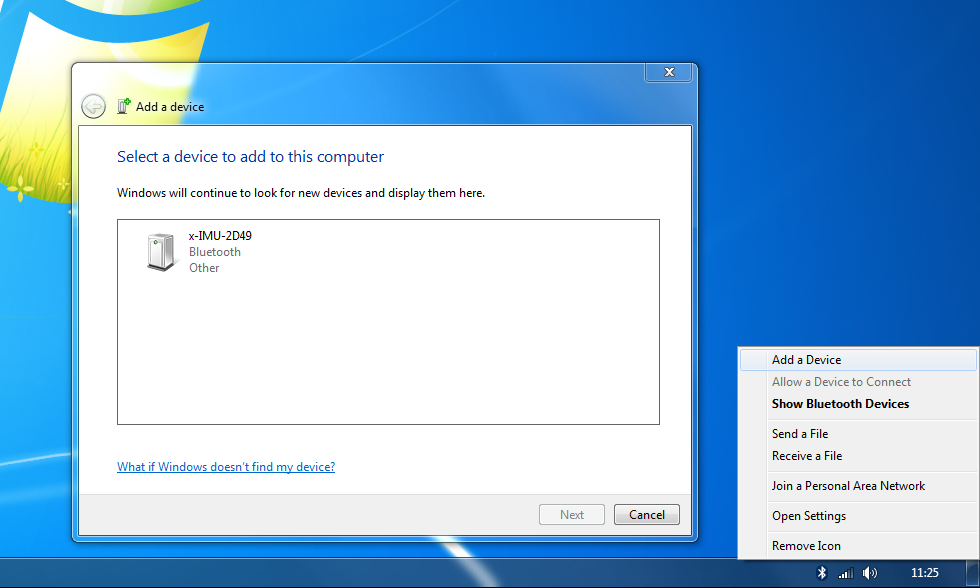
\includegraphics[width=0.7\textwidth]{graphics/AddBluetoothDeviceSearch.png}
		\caption{Searching for the x-IMU as a new Bluetooth device in Windows 7}
	\label{fig:AddBluetoothDeviceSearch}
\end{figure}

Once the x-IMU has been found by the host computer, it can be added.  This will require the user to enter the x-IMU's Bluetooth pass code: \textit{1234}.  The x-IMU Bluetooth pairing will be assigned an available serial port name by the host computer; for example \textit{COM3}.  For example, Figure \ref{fig:AddBluetoothDevicePasscode} shows this being done in Windows 7.

\begin{figure}[H]
	\centering
		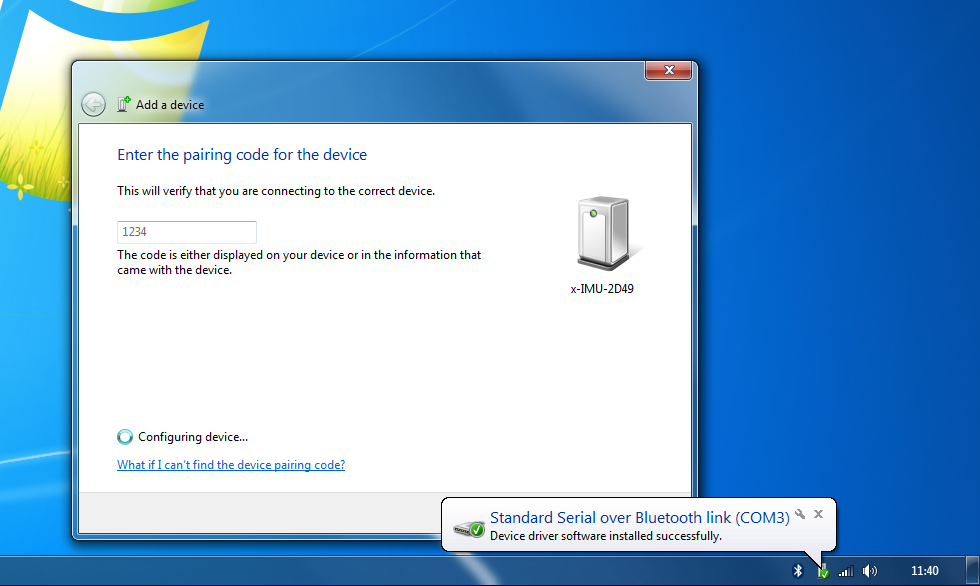
\includegraphics[width=0.7\textwidth]{graphics/AddBluetoothDevicePasscode.png}
		\caption{Adding the x-IMU as a new Bluetooth device in Windows 7}
	\label{fig:AddBluetoothDevicePasscode}
\end{figure}

The port name assigned to the x-IMU Bluetooth pairing can be confirmed at any time by viewing the services of the x-IMU.  For example, Figure \ref{fig:BluetoothServices} shows how this is done in Windows 7 having right clicked the x-IMU Bluetooth device icon.

\begin{figure}[H]
	\centering
		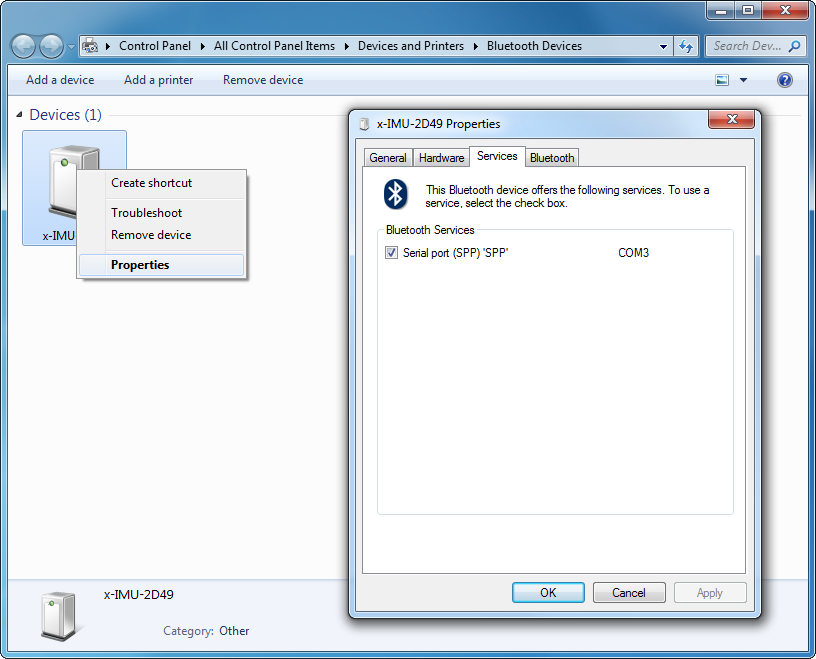
\includegraphics[width=0.6\textwidth]{graphics/BluetoothServices.png}
		\caption{Confirming the port name assigned to the x-IMU Bluetooth pairing}
	\label{fig:BluetoothServices}
\end{figure}

%---------------------------------------------------------------------------------------------------
\subsection{Bluetooth LED}
\label{sec:BluetoothLED}

The blue Bluetooth LED indicates the Bluetooth radio state.  The LED behaviour and associated Bluetooth radio states are detailed in table \ref{tab:BluetoothLEDstates}.

\begin{table}[H]
	\centering
		\begin{tabular}{l  l}
		\hline	
		LED behaviour		&	Bluetooth state\\
		\hline	
		Off							& Switched off.  Power to the radio is compeltely disconected\\			
		Flashing (1 Hz)	& Fully powered and discoverable\\
		On							& Fully powered and connected\\
		\hline
		\end{tabular}
		\caption{Bluetooth LED states}			
	\label{tab:BluetoothLEDstates}
\end{table}

%---------------------------------------------------------------------------------------------------
\subsection{Bluetooth bandwidth}
\label{sec:BluetoothBandwidth}

It is possible for the user to define data output rate settings (e.g. \ref{sec:BatteryAndThermometerDataOutputRate}, \ref{sec:InertialAndMagneticDataOutputRate}, \ref{sec:QuaternionDataOutputRate}) so that the data being generated by the x-IMU exceeds the bandwidth of a communication channel.  If the Bluetooth bandwidth is exceed, the Bluetooth transmit buffer will overrun and some data will be lost.  When this happens a \textit{Bluetooth transmit buffer overrun} error (\ref{sec:BluetoothTransmitBufferOverrun}) will be generated.  As this error message is sent immediately after the buffer has overrun, the error message will be successfully transmitted.  This error can be avoided by reducing the data output rate settings (e.g. \ref{sec:BatteryAndThermometerDataOutputRate}, \ref{sec:InertialAndMagneticDataOutputRate}, \ref{sec:QuaternionDataOutputRate}).

All data sent to the x-IMU via Bluetooth is buffered in the Bluetooth receive buffer before being processed.  The time required to process the received data is dependent on the data.  If data is sent to the x-IMU via Bluetooth at a rate at a rate greater than it can be processed then the receive buffer will overflow and some data will be lost.  When this happens a \textit{Bluetooth receive buffer overrun} error (\ref{sec:BluetoothReceiveBufferOverrun}) will be generated.

%---------------------------------------------------------------------------------------------------
\subsection{Optimising Bluetooth performance}
\label{sec:OptimisingBluetoothPerformance}

The practical range and quality of the Bluetooth connection are dependent on a number of factors.  A poor Bluetooth connection will be unable to handle higher data output rates and so result in missing data and \textit{Bluetooth transmit buffer overrun} errors  (\ref{sec:BluetoothTransmitBufferOverrun}).  The use of lower data output rate settings (e.g. \ref{sec:BatteryAndThermometerDataOutputRate}, \ref{sec:InertialAndMagneticDataOutputRate}, \ref{sec:QuaternionDataOutputRate}) can help achieve a more reliable Bluetooth communication channel.  The x-IMU uses a class I Bluetooth radio which represents a maximum range of 100 m.  However, the practical performance is limited by computer's Bluetooth class; for example a class II Bluetooth dongle (representing a range of 10 m) will limit the x-IMU's operating range to 10 m.  Performance also varies between Bluetooth dongle brands, a dongle from a  reputable brand may be expected to perform better than a low-cost budget product.  Bluetooth is a radio system and so the location of the antennae (usually built into the dongle) should be given consideration.  For example, a miniature Bluetooth dongle plugged in to the back a desktop PC can be expected to achieve worse performance than if the dongle was fixed to a front USB port with line-of-sight to the x-IMU.

%\paragraph{Using mulitple x-IMUs}
%\label{sec:UsingMulitpleXIMUs}
%A single Bluetooth host (e.g. Bluetooth dongle) can connect to up to 7 x-IMUs simultaneously.  Each x-IMU is assigned a separate serial port name and operated independently; however, the bandwidth is limited due that of the single Bluetooth host.

%=====================================================================================================
% SD card
%=====================================================================================================
\section{SD card}
\label{sec:SDCard}

The x-IMU streams all communication data simultaneously and identically via USB (\ref{sec:USB}), Bluetooth (\ref{sec:Bluetooth}) and to a file on the SD card.  The SD card may therefore be used in conjunction with the USB and/or Bluetooth or as the sole communication channel allowing the x-IMU to function as a standalone data logger.  Data is logged to the SD card on separate files binary files that are automatically created each time the x-IMU is switched on, reset or wakes up.  Logging is only then stopped once the x-IMU is reset or enters sleep mode.  The binary files (\verb=.bin=) created may be read form the SD card on to any PC and then converted to individual Comma Separated Variable (\verb=.csv=) and text (\verb=.txt=) files using via the \xIMUGUI{} \textit{SD Card} tab page (\ref{sec:TabPageSDCard}).  Alternatively the \href{http://www.x-io.co.uk/node/10#sd_card_binary_file_converter}{x-IMU Binary File Converter} may be used for command-line-based or automated conversion of multiple files.  Converted CSV and text files can be directly imported into programmes such as MATLAB and Microsoft Excel.  The \href{http://www.x-io.co.uk/node/10#matlab_import_ximu_data}{MATLAB x-IMU Library} includes all the tools required to import, structure and plot x-IMU data.

The x-IMU supports conventional SD cards and HCSD cards.  Cards may be formatted as FAT16 (usually cards equal or less than 2 GB) and FAT32 (for card greater than 2 GB).  For reliable performance it is recommended that the SD card is formatted prior to each use.

%---------------------------------------------------------------------------------------------------
\subsection{Creating and closing files}
\label{sec:CreatingAndClosingFiles}

The x-IMU automatically creates a new file on the SD card each time the x-IMU is switched on, reset or wakes up.  If an SD card is not accessible at this point, the x-IMU will not create a file and the SD card will not be used.  The new file name is created as the 5 digit number stored in the \textit{SD card new file name} register (\ref{sec:SDCardNewFileName}); for example, \verb=00000.bin=.  The number stored in this register is automatically incremented each time a new file is created.  This ensures that each file created by the x-IMU is given a unique file name until the maxium file name of \verb=65535.bin= is reached; the file name will then automatically reset to \verb=00000.bin= and start again.  The user can reset this value to any number by writing to the register (\ref{sec:SDCardNewFileName}).  If the x-IMU attempts to create a file name that already exists on the SD card, the x-IMU automatically increment the file name and try again.  If all file names have been used, the x-IMU will not create a file and the SD card will not be used.

File must be closed before the SD card is removed or the x-IMU switched off otherwise the file will be corrupted and all data written to the file will have been lost.  The file is automatically closed when the x-IMU is reset or enters sleep mode (\ref{sec:SleepMode}).  Users wishing to frequency remove the SD card may wish to have the push button (\ref{sec:PushButton}) configured in \textit{sleep/wake} mode.

%---------------------------------------------------------------------------------------------------
\subsection{SD card LED}
\label{sec:SDCardLED}

The amber SD card LED indicates SD card activity.  The LED remains lit each time a burst of data is written to the SD card.  If the user low defines data output rates then the LED will blink infrequenctly, high data output rates will mean the LED will flash rapidly.  The SD card LED therefore provides an indication of SD card bandwidth performance (\ref{sec:SDCardBandwidth}).

%---------------------------------------------------------------------------------------------------
\subsection{SD card bandwidth}
\label{sec:SDCardBandwidth}

It is possible for the user to define data output rate settings (e.g. \ref{sec:BatteryAndThermometerDataOutputRate}, \ref{sec:InertialAndMagneticDataOutputRate}, \ref{sec:QuaternionDataOutputRate}) so that the data being generated by the x-IMU exceeds the bandwidth of a communication channel.  The SD card bandwidth is greater than the USB and Bluetooth bandwidth and so the SD card may still provide reliable data logging when the USB or Bluetooth channel bandwidth is exceeded.  If the SD card bandwidth is exceed, the SD card buffer will overrun and some data will be lost.  When this happens an \textit{SD card write buffer overrun} error (\ref{sec:SDCardWriteBufferOverrun}) will be generated.  As this error packet is sent immediately after the buffer has overrun, the error message will be successfully logged to the SD card.  This error can be avoided by reducing the data output rate settings (e.g. \ref{sec:BatteryAndThermometerDataOutputRate}, \ref{sec:InertialAndMagneticDataOutputRate}, \ref{sec:QuaternionDataOutputRate}).  The SD card LED (\ref{sec:SDCardLED}) may be used to provides an indication of SD card bandwidth performance while access to error messages is not available.

The effective bandwidth of SD card varies between different SD card manufacturers and may decrease significantly if the SD card becomes fragmented.  It is therefore recommended that the SD card is formatted prior to each use.

%---------------------------------------------------------------------------------------------------
\subsection{Magnetic distortions from SD card socket}
\label{sec:MagneticDistortionsFromSDCardSocket}

The SD card socket contains a ferromagnetic mechanism that may distort magnetometer measurements in different ways dependant of the presence of an SD card.  These distortions are removed through hard-iron calibration and each x-IMU is calibrated and supplied with a dummy SD card that may be used to ensure constant SD card socket magnetic characteristics.

%=====================================================================================================
% Real-time clock and calendar
%=====================================================================================================
\section{Real-time clock and calendar}
\label{sec:RealTimeClockAndCalendar}

The on-board real-time clock and calendar provides accurate measurement of the date and time and is pre-programmed to account for leap-years between the year 2000 and 2099.  The real-time clock and calendar data can be viewed and synchronised with the computer clock using the \xIMUGUI{} via the \textit{Date/Time} tab page (\ref{sec:TabPageDateTime}).

The real-time clock and calendar data a is provided by the x-IMU in the \textit{write date/time data} packets.  The output rate of these packets of either disabled or 1 Hz is specified in the \textit{date/time data rate} register (\ref{sec:DateTimeDataOutputRate}).  A single \textit{date/time data} packet is always sent on device reset regardless of user settings so that the date and time are is hardcoded as the first packet written to the SD card (\ref{sec:SDCard}).  The real-time clock and calendar is set by sending a \textit{write date/time data} packet to the x-IMU, once the new date and time have been set the x-IMU will respond with a \textit{write date/time data} containing the real-time clock and calendar data.  This data may also be requested by sending a \textit{read date/time data} packet to the x-IMU.

%---------------------------------------------------------------------------------------------------
\subsection{Maintaining clock power}
\label{sec: Maintaining ClockPower}

The real-time clock and calendar require power to operate.  If power is lost for the x-IMU switch off then the date and time will reset to 01/01/2000 00:00:00.  Applications that require date and time to be maintained should ensure that the x-IMU is never switched off and instead take advantage of sleep mode (\ref{sec:SleepMode}).

%=====================================================================================================
% Sensors
%=====================================================================================================
\section{Sensors}
\label{sec:Sensors}

The x-IMU's on-board sensors include a triple axis gyroscope, triple axis accelerometer, triple axis magnetometer, thermometer and a battery voltmeter.  The user may access individual sensor data as either \textit{Raw un-calibrated ADC results} or as \textit{Calibrated units} by specifying the mode in the \textit{Sensor data mode} register (\ref{sec:SensorDataMode}).  The data from individual sensors is proved in either the \textit{Raw inertial/magnetic data} and \textit{Raw battery and thermometer data} packets or the \textit{Calibrated inertial/magnetic data} and \textit{Calibrated battery and thermometer data} packets.  The output rate of these packets of up to 256 Hz is specified in the \textit{Battery and thermometer data output rate} (\ref{sec:BatteryAndThermometerDataOutputRate}) and \textit{Inertial/magnetic data output rate} (\ref{sec:InertialAndMagneticDataOutputRate}) registers.

%---------------------------------------------------------------------------------------------------
\subsection{Battery voltmeter}
\label{sec:BatteryVoltmeter}

The battery voltmeter allows the battery voltage to be monitored by the user application.  The battery voltmeter must be correctly calibrated if the low battery voltage detection functionality is to be used.  The battery voltmeter has 12-bit resolution and a range of 0 V to  6.6 V.  When the power switch is in the \textit{off} position (so that the x-IMU may be powered from an external source via the auxiliary port) the battery voltmeter will instead measure the voltage of the external source.

\paragraph{Raw ADC data:}
In raw data mode the battery voltmeter data is the ADC integer value between 0 and 4096 corresponding to a voltage between 0 V and 6.6 V.  This data is provided in the \textit{Raw battery and thermometer data} packets.

\paragraph{Calibrated data:}
In calibrated data mode the battery voltmeter data is the calibrated measurement in Volts.  This data is provided in the \textit{Calibrate battery and thermometer data} packets.  The calibrated measurement $v$ is calculated from the raw ADC measurements $\tilde{v}$ according to a sensitivity $s_v$ and bias $b_v$ as described by equation \eqref{batteryCal}.  Parameters $b_v$ and $s_v$ are defined in the battery voltmeter sensitivity (\ref{sec:BatteryVoltmeterSensitivity}) and bias (\ref{sec:BatteryVoltmeterBias}) registers.

\begin{equation}
	v = \frac{1}{s_v} ( \tilde{v} - b_v )
	\label{batteryCal}
\end{equation}


%---------------------------------------------------------------------------------------------------
\subsection{Thermometer}
\label{sec:Thermometer}

The thermometer is built in to the gyroscope and provides a measurement of the temperature of the device. The thermometer must be correctly calibrated for calibrated gyroscope measurements to compensate for gyroscope bias temperature sensitivity.  The thermometer has 16-bit resolution and has a range of -30$^{\circ}$C to +85$^{\circ}$C.  See the \gyroName{} datasheet for further information on the thermometer's characteristics.

\paragraph{Raw ADC data:}
In raw data mode the thermometer data is the ADC integer value between $-32,768$ and $+32,767$ linearly proportional to temperature.  This data is provided in the \textit{Raw battery and thermometer data} packets.

\paragraph{Calibrated data:}
In calibrated data mode the thermometer data is the calibrated temperature in $^{\circ}$C.  This data is provided in the \textit{Calibrate battery and thermometer data} packets.  The calibrated measurement $\tau$ is calculated from the raw ADC measurement $\tilde{\tau}$ according to a defined sensitivity $s_\tau$ and bias $b_\tau$ as described by equation \eqref{thermCal}.  Parameters $b_\tau$ and $s_\tau$ are defined in the battery voltmeter sensitivity (\ref{sec:ThermometerSensitivity}) and bias (\ref{sec:ThermometerBias}) registers.

\begin{equation}
	\tau = \frac{1}{s_\tau} ( \tilde{\tau} - b_\tau )
	\label{thermCal}
\end{equation}

%---------------------------------------------------------------------------------------------------
\subsection{Gyroscope}
\label{sec:Gyroscope}

The triple axis gyroscope provides a measurement of the angular velocities around the $x$, $y$ and $z$ axes of the x-IMU.  The gyroscope must be correctly calibrated in order for the IMU and AHRS algorithms to be able to function correctly; the algorithms use measurements of angular velocities to filter out errors in the estimated orientation caused by linear accelerations and temporal magnetic distortions.  The gyroscope has 16-bit resolution and a range of $\pm2000^{\circ}$/s.  See the \gyroName{} datasheet for further information on the gyroscope's characteristics.

\paragraph{Raw ADC data:}
In raw data mode the gyroscope data is the ADC integer values between $-32,768$ and $+32,767$ linearly proportional to angular velocities.  This data is provided in the \textit{Raw inertial/magnetic data} packets.

\paragraph{Calibrated data:}
In calibrated data mode the gyroscope data are calibrated angular velocities in $^{\circ}$/s.  This data is provided in the \textit{Calibrated inertial/magnetic data} packets.  The calibrated measurements $g_x$, $g_y$ and $g_z$ are calculated from the raw ADC measurements $\tilde{g}_x$, $\tilde{g}_y$ and $\tilde{g}_z$ according to the defined sensitivities $s_{g_x}$, $s_{g_y}$ and $s_{g_z}$, temperature of the device $\tau$, biases at 25$^{\circ}$C $b_{g_x}$, $b_{g_y}$ and $b_{g_z}$ and bias temperature sensitivities $f_x$, $f_y$ and $f_z$.  The calibrated measurmndts are described by equation \eqref{gyroCal}.  Parameters $s_{g_x}$, $s_{g_y}$, $s_{g_z}$, $b_{g_x}$, $b_{g_y}$, $b_{g_z}$, $f_x$, $f_y$ and $f_z$ are defined in the separate gyroscope calibration parameter registers (\ref{sec:GyroscopeXAxisSensitivity} to \ref{sec:GyroscopeZAxisBiasTemperatureSensitivity}).

\begin{equation}
	\begin{bmatrix}
		g_x\\
		g_y\\
		g_z
	\end{bmatrix}
	=
	\begin{bmatrix}
		s_{g_x}	& 0				& 0				\\
		0				& s_{g_y}	&	0				\\
		0				& 0 			& s_{g_z}
	\end{bmatrix}		
	^{-1}
	\left(
	\begin{bmatrix}
		\tilde{g}_x\\
		\tilde{g}_y\\
		\tilde{g}_z
	\end{bmatrix}	
	-
	\begin{bmatrix}
		b_{g_x}\\
		b_{g_y}\\
		b_{g_z}
	\end{bmatrix}
	-
	\begin{bmatrix}
		f_x	& 0				& 0			\\
		0				& f_y	&	0			\\
		0				& 0 	& f_z
	\end{bmatrix}		
	^{-1}
	\begin{bmatrix}
		\tau - 25\\
		\tau - 25\\
		\tau - 25
	\end{bmatrix}	
	\right)
	\label{gyroCal}
\end{equation}


%---------------------------------------------------------------------------------------------------
\subsection{Accelerometer}
\label{sec:Accelerometer}

The triple axis accelerometer and provides a measurement of the accelerations along the $x$, $y$ and $z$ axes of the x-IMU.  The accelerometer must be correctly calibrated in order for the IMU and AHRS algorithms to be able to function correctly; the algorithms use the accelerometer to measure the direction of gravity and provide an absolute reference for the pitch and roll components of the estimated orientation.  The acceleroemter has 12-bit resolution and selectable ranges from $\pm2$ g to $\pm8$ g.  The measurement range of the accelerometer is defined in \textit{Accelerometer full scale} register (\ref{sec:AccelerometerFullScale}).  See the \accelMagName{} datasheet for further information on the accelerometer's characteristics.

\paragraph{Raw ADC data:}
In raw data mode the accelerometer data is the ADC integer values between $-4096$ and $+4095$ linearly proportional to accelerations.  This data is provided in the \textit{Raw inertial/magnetic data} packets.

\paragraph{Calibrated data:}
In calibrated data mode the accelerometer data are calibrated accelerations in $g$.  This data is provided in the \textit{Calibrated inertial/magnetic data} packets.  The calibrated measurements $a_x$, $a_y$ and $a_z$ is calculated from the raw ADC measurements $\tilde{a}_x$, $\tilde{a}_y$ and $\tilde{a}_z$ according to the defined sensitivities $s_{a_x}$, $s_{a_y}$ and $s_{a_z}$ and biases $b_{a_x}$, $b_{a_y}$ and $b_{a_z}$ as described by equation \eqref{accelCal}.  Parameters $s_{a_x}$, $s_{a_y}$, $s_{a_z}$, $b_{a_x}$, $b_{a_y}$ and $b_{a_z}$ are defined in the separate accelerometer calibration parameter registers (\ref{sec:AccelerometerXAxisSensitivity} to \ref{sec:AccelerometerZAxisBias}).  The sensitivities and biases will be different for each full-scale measurement range (\ref{sec:AccelerometerFullScale}).

\begin{equation}
	\begin{bmatrix}
		a_x\\
		a_y\\
		a_z
	\end{bmatrix}
	=
	\begin{bmatrix}
		s_{a_x}	& 0				& 0				\\
		0				& s_{a_y}	&	0				\\
		0				& 0 			& s_{a_z}
	\end{bmatrix}		
	^{-1}
	\left(
	\begin{bmatrix}
		\tilde{a}_x\\
		\tilde{a}_y\\
		\tilde{a}_z
	\end{bmatrix}	
	-
	\begin{bmatrix}
		b_{a_x}\\
		b_{a_y}\\
		b_{a_z}
	\end{bmatrix}		
	\right)
	\label{accelCal}
\end{equation}


%---------------------------------------------------------------------------------------------------
\subsection{Magnetometer}
\label{sec:Magnetometer}

The triple axis magnetometer and provides a measurement of the magnetic flux along the $x$, $y$ and $z$ axes.  The magnetometer must be correctly calibrated in order for the AHRS algorithm to be able to function correctly; the algorithm uses the magnetometer to measure the Earth's magnetic field and provide an absolute reference for the heading component of the estimated orientation.    The magnetometer has 12-bit resolution and selectable ranges from $\pm1.3$ G to $\pm8.1$ G.  The measurement range of the magnetometer is defined in \textit{Magnetometer full scale} register (\ref{sec:MagnetometerFullScale}).  See the \accelMagName{} datasheet for further information on the magnetometer's characteristics.

\paragraph{Raw ADC data:}
In raw data mode the magnetometer data is the ADC integer values between $-4096$ and $+4095$ linearly proportional to magnetic flux.  This data is provided in the \textit{Raw inertial/magnetic data} packets.  A value fo -4096 will be provided when the measurement saturates in either direction.

\paragraph{Calibrated data:}
In calibrated data mode the magnetometer data are calibrated accelerations in $G$.  This data is provided in the \textit{Calibrated inertial/magnetic data packets}.  The calibrated measurements $m_x$, $m_y$ and $m_z$ are calculated from the raw ADC measurements $\tilde{m}_x$, $\tilde{m}_y$ and $\tilde{m}_z$ according to the defined sensitivities $s_{m_x}$, $s_{m_y}$ and $s_{m_z}$, biases $b_{m_x}$, $b_{m_y}$ and $b_{m_z}$ and hard-iron biases $h_x$, $h_y$ and $h_z$ as described by equation \eqref{magCal}.  Parameters $s_{m_x}$, $s_{m_y}$, $s_{m_z}$, $b_{m_x}$, $b_{m_y}$, $b_{m_z}$, $h_x$, $h_y$ and $h_z$ are defined in the separate magnetometer calibration parameter registers (\ref{sec:MagnetometerXAxisSensitivity} to \ref{sec:MagnetometerZAxisHardIronBias}).  The sensitivities and biases will be different for each full-scale measurement range (\ref{sec:MagnetometerFullScale}).

\begin{equation}
	\begin{bmatrix}
		m_x\\
		m_y\\
		m_z
	\end{bmatrix}
	=
	\begin{bmatrix}
		s_{m_x}	& 0				& 0				\\
		0				& s_{m_y}	&	0				\\
		0				& 0 			& s_{m_z}
	\end{bmatrix}		
	^{-1}
	\left(
	\begin{bmatrix}
		\tilde{m}_x\\
		\tilde{m}_y\\
		\tilde{m}_z
	\end{bmatrix}	
	-
	\begin{bmatrix}
		b_{m_x}\\
		b_{m_y}\\
		b_{m_z}
	\end{bmatrix}	
	\right)		
	-
	\begin{bmatrix}
		h_x\\
		h_y\\
		h_z
	\end{bmatrix}			
	\label{magCal}
\end{equation}

\newpage
%=====================================================================================================
% Sensor calibration
%=====================================================================================================
\section{Sensor calibration}
\label{sec:SensorCalibration}

\sectionComingSoon{}

%The sensors must be correctly calibrated for the IMU and AHRS algorithms to provide an accurate estimate of orientation.  The battery voltmeter must be correctly calibrated for the low battery voltage detection functionality to work properly.
%
%...save registers when done
%
%... For accurate calibration users should calibrate the x-IMU while it is in its intedned state...
%... all register settings... SD card connected or not...
%
%
%Each x-IMU is supplied pre-calibrated to provide an acceptable level of perfomrance for most user applcaitons.  All calibration parameters are defined in the registers ()
%
%
%%\subsection{When to re-calibrate}
%%\label{sec:WhenToReCalibrate}
%%
%%It is recommended that the user re-calibrated all sensors once the x-IMU is installed within its final application.  Doing so will ensure that any changes to sensor characteristics due to mechanical stresses, operating temperature range, mechanical stresses or magnetic environment, are accounted for by calibration.
%%
%%\paragraph{Changes to temperture:}
%%
%%\paragraph{Changes to mechancial stresses:} Mechcanical stresses to the x-IMU may cause changes to sensor characterstics.  The gyroscope bias is particaully sensitve to mechaicnal stresses.
%%
%%\paragraph{Changes to magnetic characterstics:}
%%
%%SD card.
%
%%------------------------------------------------
%\subsection{Gyroscope calibration}
%\label{sec:GyroscopeCalibration}
%
%
%The gyroscope calibration model used by the x-IMU and described in section \ref{sec:Gyroscope} requires that values for the sensitivities $s_{g_x}$, $s_{g_y}$ and $s_{g_z}$, biases at 25$^{\circ}$C $b_{g_x}$, $b_{g_y}$ and $b_{g_z}$ and bias temperature sensitivities $f_x$, $f_y$ and $f_z$ are defined within the gyroscope calibration registers (\ref{sec:GyroscopeXAxisSensitivity} to \ref{sec:GyroscopeZAxisBiasTemperatureSensitivity}).
%
%\paragraph{Gyroscope sensitivities}
%\label{sec:GyroscopeSensitivities}
%The sensitivities $s_{g_x}$, $s_{g_y}$ and $s_{g_z}$ are pre-calibrated by the gyroscope manufacturer.  The typical values quoted in the gyroscope datasheet are used by all x-IMUs and will provide sufficient accuracy for most user applications.  See the \gyroName{} datasheet for specific details on these parameters.
%
%\paragraph{Gyroscope biases}
%\label{sec:GyroscopeBiases}
%The gyroscope biases at 25$^{\circ}$C $b_{g_x}$, $b_{g_y}$ and $b_{g_z}$ and bias temperature sensitivities $f_x$, $f_y$ and $f_z$ vary between different x-IMUs and are uniquely calibrated for each unit using the on-board gyroscope bias calibration algorithm (\ref{sec:GyroscopeBiasCalibraitonAlgorithm}).  The gyroscope biases parameters are extrmely senstive to mechanical strain affecting the PCB.
%
%%---------------------------------------------------------------------------------------------------
%\subsubsection{Gyroscope bias calibraiton algorithm}
%\label{sec:GyroscopeBiasCalibraitonAlgorithm}
%
%The
%
%- x-IMU warms up while switched on andits operating tempreture may depend of settings and usage.
%
%%---------------------------------------------------------------------------------------------------
%\subsection{Accelerometer calibration}
%\label{sec:AccelerometerCalibration}
%
%The acceleroemter calibration model used by the x-IMU and described in section \ref{sec:Accelerometer} requires that values for the sensitivities $s_{a_x}$, $s_{a_y}$ and $s_{a_z}$ and biases $b_{a_x}$, $b_{a_y}$ and $b_{a_z}$ are defined within the accelerometer calibration registers (\ref{sec:AccelerometerXAxisSensitivity} to \ref{sec:AccelerometerZAxisBias}).
%
%\paragraph{Accelerometer sensitivities}
%\label{sec:AccelerometerSensitivities}
%
%
%
%%---------------------------------------------------------------------------------------------------
%\subsection{Magnetometer calibration}
%\label{sec:MagnetometerCalibration}
%
%...
%
%%---------------------------------------------------------------------------------------------------
%\subsubsection{Magnetometer calibraiton algorithm}
%\label{sec:MagnetometerCalibraitonAlgorithm}
%
%...
%
%%------------------------------------------------
%\subsubsection{Hard-iron calibration}
%\label{sec:HardIronCalibration}
%
%...

\newpage
%=====================================================================================================
% IMU/AHRS algorithms
%=====================================================================================================
\section{IMU/AHRS algorithms}
\label{sec:IMUAHRSAlgorithms}

\sectionComingSoon{}

%The on-board sensor fusion algorithm uses the gyroscope, accelerometer and magnetometer to provide an optimal, real-time estimate of the devices' orientation relative to the Earth.  The IMU and AHRS algorithms require that the on-board sensors are properly calibrated (\ref{sec:Calibration}).  The estimated orientation is represented as a quaternion and is transmitted in the quaternion data packet \ref{sec:QuaternionData}.  The algorithm internal update rate is fixed at 256 Hz regardless of the quaternion data output rate (\ref{sec:QuaternionDataOutputRate}).
%
%
%%---------------------------------------------------------------------------------------------------
%\subsection{Algorithm modes}
%\label{sec:AlgorithmModes}
%
%The algorithm can run in either IMU (Inertial Measurement Unit) or AHRS (Attitude Heading Reference System) mode (\ref{sec:AlgorithmMode}).
%
%\paragraph{IMU mode}
%\label{sec:IMUMode}
%In IMU mode, only the gyroscope and accelerometer are used.  In this mode, the heading component of the estimated orientation will be subject to integral drift so that only the pitch and roll components may be trusted to be accurate.  The advantage using IMU mode is that magnetic measurements are completely ignored and so cannot corrupt the estimated orientation.  This is of use in applications that only require the pitch and roll components of a measured orientation; for example, camera stabilisation.
%
%\paragraph{AHRS mode}
%\label{sec:AHRSMode}
%In AHRS mode, the gyroscope, accelerometer and magnetometer are all used.  In this mode the estimated orientation is not subject to any integral drift.
%
%
%%---------------------------------------------------------------------------------------------------
%\subsection{Algorithm gains}
%\label{sec:AlgorithmGains}
%
%\paragraph{Proportional gain}
%\label{sec:ProportionalGain}
%The proportional feedback gain governs the rate at which the algorithm output converges to an orientation assumed by the accelerometer (in IMU mode) and magnetometer (in AHRS mode) measurements.  A large gain will mean that the estimated orientation will converge quickly and so will result in a 'shaky' orientation that is corrupted by linear accelerations and temporal magnetic distortions.  A low gain will mean that the estimated orientation 'trust the gyroscopes more' and result in a 'smooth' orientation; however, the algorithm will be less able to compensate for errors in the gyroscope measurements and calibration.  If a proportional gain of zero is used, then accelerometer and magnetometer measurements are completely ignored.
%
%\paragraph{Integral gain}
%\label{sec:IntegralGain}
%...
%
%%---------------------------------------------------------------------------------------------------
%\subsection{Algorithm operations}
%\label{sec:AlgorithmOperations}
%
%%------------------------------------------------
%\subsubsection{Reset algorithm}
%\label{sec:ResetAlgorithm}
%
%%------------------------------------------------
%\subsubsection{Tare}
%\label{sec:Tare}
%
%%------------------------------------------------
%\subsubsection{Clear tare}
%\label{sec:ClearTare}

%%---------------------------------------------------------------------------------------------------
%\subsection{Algorithm operations}
%\label{sec:AlgorithmOperations}
%
% OPTIMISING ALGORITHM PEROFRMANCE!!!


\newpage
%=====================================================================================================
% Power management
%=====================================================================================================
\section{Power management}
\label{sec:PowerManagement}

The x-IMU may be powered via USB (\ref{sec:USB}), an external supply (\ref{sec:ExternalSupply}) or a single cell lithium polyer (LiPo) battery cell (\ref{sec:BatteryAndCharging}).

%---------------------------------------------------------------------------------------------------
\subsection{External supply}
\label{sec:ExternalSupply}

The x-IMU may be powered by a 3.5 to 7.7 V external supply via the auxiliary port (\ref{sec:AuxiliaryPort}).  The supply should be connected to the \textit{GND} and \textit{EXT} pins.  This power supply is only enabled while the power switch (\ref{sec:PowerSwitch}) is in the \textit{off} position.  In this situation, the battery volt meter (\ref{sec:BatteryVoltmeter}) will measure the voltage of the external supply.

%---------------------------------------------------------------------------------------------------
\subsection{Battery and charging}
\label{sec:BatteryAndCharging}

The x-IMU has a standard connector for a 3.7 V single cell Lithium Polymer (LiPo) battery cell.  These batteries are widely available in range of capacities, for example \href{http://www.sparkfun.com/products/339}{1000 mAh} and \href{http://www.sparkfun.com/products/8483}{2000 mAh}.  The battery life is dependent on user settings and usage.  See the tips on minimising power consumption section (\ref{sec:TipsForMinimisingPowerConsumption}).

The x-IMU has an on-board battery charger specially designed for LiPo battery cells.  The battery is charged automatically while the x-IMU is connected to a USB port.  The red charging LED (\ref{sec:ChargingLEDRed}) will remain lit while the battery is charging.  Charging stops automatically once complete.  The x-IMU may be used as normal while the battery is charging.  It is not necessary for the connected computer to have the USB drivers installed for charging; however, the charging process will be faster if the drivers are installed.

%---------------------------------------------------------------------------------------------------
\subsection{Low battery voltage detection}
\label{sec:LowBatteryVoltageDetection}

The calibrated battery voltmeter (\ref{sec:BatteryVoltmeter}) is used to trigger sleep mode (\ref{sec:SleepMode}) once the battery voltage falls below a specific level defined in the \textit{battery shutdown voltage} register (\ref{sec:BatteryShotdownVoltage}).  This allows the x-IMU to execute critical tasks prior to power failure; for example closing the file on the SD card and notifying the user or host software of the situation (\ref{sec:LowBattery}).  By entering sleep mode prior to power failure, the x-IMU also ensures that the date and time of the real-time clock and calendar (\ref{sec:RealTimeClockAndCalendar}) are not lost.  The low battery voltage detection is disabled while USB is connected.

%---------------------------------------------------------------------------------------------------
\subsection{Sleep mode}
\label{sec:SleepMode}

In sleep mode, the x-IMU remains powered but all on-board components are shutdown.  This allows the device to be effectively `turned off' without disabling power to essential components; for example, the real time clock and calendar (\ref{sec:RealTimeClockAndCalendar}).  The green status LED (\ref{sec:StatusLEDGreen}) will blink once every 3 seconds to indicate that the device is in sleep mode.  Sleep mode is enabled through the sources listed below.  The x-IMU will reset upon wake up so that the same behaviour may be expected when the devices is powered on, reset or awakened.  The wake up sources are listed below.
  
\paragraph{Sleep mode enable sources:}
\label{sec:SleepModeEnableSources}

\begin{itemize}
	\item Push button (\ref{sec:PushButton}) in \textit{sleep/wake} mode
	\item Sleep command via USB or Bluetooth
	\item Low battery voltage detection (\ref{sec:LowBatteryVoltageDetection})
	\item Sleep timer (\ref{sec:SleepTimer})
\end{itemize}

\paragraph{Wake up sources}
\label{sec:WakeUpSources}

\begin{itemize}
	\item Push button (\ref{sec:PushButton}) in sleep/wake mode
	\item Motion trigger wake up (\ref{sec:MotionTriggeredWakeUp})
\end{itemize}

%---------------------------------------------------------------------------------------------------
\subsection{Sleep timer}
\label{sec:SleepTimer}

The sleep timer will trigger sleep mode after the period of time defined in the \textit{sleep timer} register (\ref{sec:SleepTimerReg}) has elapsed.  The sleep timer countdown starts when the x-IMU starts up and may be reset by the sources listed below.  These sources enable the detection of motion, the user or the host software to prevent the x-IMU from entering sleep mode.  The sleep timer is disabled by specifying a \textit{sleep timer} register (\ref{sec:SleepTimerReg}) value of 0 seconds.  The sleep timer is disabled while USB is connected.

\paragraph{Sleep timer reset sources}
\label{sec:SleepTimerResetSources}

\begin{itemize}
	\item \textit{Reset sleep timer} command (\ref{sec:ResetSleepTimer})
	\item Motion trigger wake up (\ref{sec:MotionTriggeredWakeUp})
\end{itemize}

%---------------------------------------------------------------------------------------------------
\subsection{Motion triggered wake up}
\label{sec:MotionTriggeredWakeUp}

The motion trigger wake up is enabled via the \textit{motion trigger wake up} register (\ref{sec:MotionTriggerWakeUp}) and may be either disabled or set to a \textit{low} or high \textit{sensitivity}.  Motion is detected using accelerometer.  If motion is detected while the x-IMU is in sleep mode then the x-IMU will wake up.  While the x-IMU is not in sleep mode the motion trigger wake up is used to reset the sleep timer (\ref{sec:SleepTimerReg}) and thus postpone sleep while motion persists.  For example, if the sleep timer is set to 20 seconds and there is sufficient motion once every 10 seconds the motion trigger wake up will prevent the sleep timer from expiring.

%---------------------------------------------------------------------------------------------------
\subsection{Tips for minimising power consumption}
\label{sec:TipsForMinimisingPowerConsumption}

Battery powered applications require that power consumption is minimised in order to extend the battery life.  The x-IMU is designed to optimised power consumption according to user settings.  The user may therefore expect a considerable reduction in power consumption and extended battery life simply by using register settings appropriate to their application.

\paragraph{Tips}
\label{sec:Tips}

\begin{itemize}
	\item Set data rates of unused data to \textit{Disabled}.
	\item Use the minimum data rates required by application.
	\item Set IMU/AHRS algorithm (\ref{sec:IMUAHRSAlgorithms}) mode to \textit{Disabled} if not required.
	\item Disable Bluetooth (\ref{sec:Bluetooth}) if not required.
	\item Use the sleep timer (\ref{sec:SleepTimer}) and motion trigger wake up (\ref{sec:MotionTriggeredWakeUp}) to automatically enter sleep mode during periods of inactivity.
\end{itemize}

\newpage
%=====================================================================================================
% Auxiliary port
%=====================================================================================================
\section{Auxiliary port}
\label{sec:AuxiliaryPort}

\sectionComingSoon{}

%Toby electronics part number
%
%\subsection{Digital I/O mode}
%\label{sec:DigitalIOMode}


\newpage
%=====================================================================================================
% Communication protocol
%=====================================================================================================
\section{Communication protocol}
\label{sec:CommunicationProtocol}

This section is currently unavailable.  Users wishing to develop their own x-IMU communication interface are advised to study the open source \xIMUAPI{} (\ref{sec:xIMUAPI}).  The API is source code is written in C\# and well commented; porting the API (or aspects of) to another language should be a straight forward exercise.

%%---------------------------------------------------------------------------------------------------
%\subsection{Packet encoding}
%\label{sec:PacketEncoding}
%
%This section is incomplete.  Please contact \verb=www.x-io.co.uk= for the document to be updated.
%
%%---------------------------------------------------------------------------------------------------
%\subsection{Checksum}
%\label{sec:Checksum}
%
%This section is incomplete.  Please contact \verb=www.x-io.co.uk= for the document to be updated.
%
%%---------------------------------------------------------------------------------------------------
%\subsection{Packet types}
%\label{sec:PacketTypes}
%
%%------------------------------------------------
%\subsubsection{Error message}
%\label{sec:ErrorMessage}
%
%This section is incomplete.  Please contact \verb=www.x-io.co.uk= for the document to be updated.
%
%%------------------------------------------------
%\subsubsection{Command message}
%\label{sec:CommandMessage}
%
%This section is incomplete.  Please contact \verb=www.x-io.co.uk= for the document to be updated.
%
%%------------------------------------------------
%\subsubsection{Read register}
%\label{sec:ReadRegister}
%
%This section is incomplete.  Please contact \verb=www.x-io.co.uk= for the document to be updated.
%
%%------------------------------------------------
%\subsubsection{Write register}
%\label{sec:WriteRegister}
%
%This section is incomplete.  Please contact \verb=www.x-io.co.uk= for the document to be updated.
%
%%------------------------------------------------
%\subsubsection{Raw battery and thermometer data}
%\label{sec:RawBatteryAndThermometerData}
%
%This section is incomplete.  Please contact \verb=www.x-io.co.uk= for the document to be updated.
%
%%------------------------------------------------
%\subsubsection{Calibrated battery and thermometer data}
%\label{sec:CalibratedBatteryAndThermometerData}
%
%This section is incomplete.  Please contact \verb=www.x-io.co.uk= for the document to be updated.
%
%%------------------------------------------------
%\subsubsection{Raw inertial and magnetic data}
%\label{sec:RawInertialAndMagneticData}
%
%This section is incomplete.  Please contact \verb=www.x-io.co.uk= for the document to be updated.
%
%%------------------------------------------------
%\subsubsection{Calibrated inertial and magnetic data}
%\label{sec:CalibratedInertialAndMagneticData}
%
%This section is incomplete.  Please contact \verb=www.x-io.co.uk= for the document to be updated.
%
%%------------------------------------------------
%\subsubsection{Quaternion data}
%\label{sec:QuaternionData}
%
%This section is incomplete.  Please contact \verb=www.x-io.co.uk= for the document to be updated.


\newpage
%=====================================================================================================
% Commands
%=====================================================================================================
\section{Commands}
\label{sec:Commands}

Commands are executed by either sending a \textit{command} packet to the x-IMU or by pressing the push button which may be configured to execute a specific command.  Commands may be send using the \xIMUGUI{} via the \textit{Commands} tab page (\ref{sec:TabPageCommands}).  Once a command has been executed the x-IMU will echo the \textit{command} packet back to the host computer as confirmation.
%The x-IMU will not process any more received data until the command has completed, this may cause recevie buffer overrun errors (\ref{sec:USBReceiveBufferOverrun}, \ref{sec:BluetoothReceiveBufferOverrun}) if the host computer continues to transmit data 
As all communication from the x-IMU to the host computer is logged to the SD card (\ref{sec:SDCard}), all command confirmations will be logged on the SD card.  If a \textit{command} packet is sent containing an invalid command code the x-IMU will respond with an \textit{invalid command} error message (\ref{sec:InvalidCommand}).

Sending a \textit{command} packet to the x-IMU will cause the x-IMU to momentarily pause sensor sampling and processing while the packet is processed.  This may cause discrepancies in the otherwise fixed data output rates.

% And data will not be processed while packet being dealt with.  THis may cause recieve buffer overrun errors.

%---------------------------------------------------------------------------------------------------
\subsection{Individual commands}
\label{sec:IndividualCommands}

%------------------------------------------------
\subsubsection{Null command}
\label{sec:NullCommand}

\begin{tabular*}{1.0\textwidth}{lp{0.815\textwidth} l}
	\textit{Command code:}	& \verb=0x0000=\\			
	\textit{Description:}	& A \textit{null command} is a valid command code but will result in no action.  As all commands sent to the x-IMU are echoed back to the sender, a null command may be used by the host software to confirm communication with the x-IMU.
\end{tabular*}

%------------------------------------------------
\subsubsection{Reset}
\label{sec:Reset}

\begin{tabular*}{1.0\textwidth}{lp{0.815\textwidth} l}
	\textit{Command code:}	& \verb=0x0001=\\			
	\textit{Description:}	& A \textit{reset} command causes a software reset of the x-IMU.  The x-IMU will close any open files on the SD card before reset, in this way the reset command may be of use to users wishing to break up a logging session into multiple files.  The reset command is used put the x-IMU into bootloader (\ref{sec:Bootloader}) mode in order to upload new firmware.  A \textit{reset} command is sent by the x-IMU to the host computer as confirmation of reset, power on and wake up.
\end{tabular*}

%------------------------------------------------
\subsubsection{Sleep}
\label{sec:Sleep}

\begin{tabular*}{1.0\textwidth}{lp{0.815\textwidth} l}
	\textit{Command code:}	& \verb=0x0002=\\			
	\textit{Description:}	& A \textit{sleep} command will put the device into sleep mode (\ref{sec:SleepMode}).  The x-IMU will close any open files on the SD card before entering sleep mode.  The x-IMU may be taken out of sleep mode by using the push button configured in \textit{sleep/wake} mode or using the motion triggered wake up functionality (\ref{sec:MotionTriggeredWakeUp}).
\end{tabular*}

%------------------------------------------------
\subsubsection{Reset sleep timer}
\label{sec:ResetSleepTimer}

\begin{tabular*}{1.0\textwidth}{lp{0.815\textwidth} l}
	\textit{Command code:}	& \verb=0x0003=\\			
	\textit{Description:}	& The \textit{reset sleep timer} command will reset the sleep timer (\ref{sec:SleepTimer}) countdown and so postpone sleep.  An example usage of this command is to create behaviour where the x-IMU will automatically enter sleep mode when communication with the host software ends or connection is lost.
\end{tabular*}

%------------------------------------------------
\subsubsection{Sample gyroscope bias at temperature 1}
\label{sec:SampleGyroscopeBiasAtTemperature1}

\begin{tabular*}{1.0\textwidth}{lp{0.815\textwidth} l}
	\textit{Command code:}	& \verb=0x0004=\\			
	\textit{Description:}	& The \textit{sample gyroscope bias at temperature 1} command is used to calibrate the gyroscope bias parameters.  This command should be sent while the x-IMU is stationary and at the lowest temperature the device is required to operate at.  The x-IMU will measure the mean temperature and gyroscope output over approximately  16 seconds, store the results to registers (\ref{sec:GyroscopeSample1Temperature} to \ref{sec:GyroscopeSample1ZAxisBias}) and then trigger a \textit{calculate gyroscope bias parameters} command (\ref{sec:CalculateGyroscopeBiasParameters}).  The execution of this command will be aborted if a \textit{gyroscope not stationary} error (\ref{sec:GyroscopeNotStationary}) occurs.  See the gyroscope calibration section for more information (\ref{sec:GyroscopeCalibration}).
\end{tabular*}

%------------------------------------------------
\subsubsection{Sample gyroscope bias at temperature 2}
\label{sec:SampleGyroscopeBiasAtTemperature2}

\begin{tabular*}{1.0\textwidth}{lp{0.815\textwidth} l}
	\textit{Command code:}	& \verb=0x0005=\\			
	\textit{Description:}	& The \textit{sample gyroscope bias at temperature 2} command is used to calibrate the gyroscope bias parameters.  This command should be sent while the x-IMU is stationary and at the highest temperature the device is required to operate at.  The x-IMU will measure the mean temperature and gyroscope output over approximately 16 seconds, store the results to registers (\ref{sec:GyroscopeSample2Temperature} to \ref{sec:GyroscopeSample2ZAxisBias}) and then trigger a \textit{calculate gyroscope bias parameters} command (\ref{sec:CalculateGyroscopeBiasParameters}).The execution of this command will be aborted if a \textit{gyroscope not stationary} error (\ref{sec:GyroscopeNotStationary}) occurs.  See the gyroscope calibration section for more information (\ref{sec:GyroscopeCalibration}).
\end{tabular*}

%------------------------------------------------
\subsubsection{Calculate gyroscope bias parameters}
\label{sec:CalculateGyroscopeBiasParameters}

\begin{tabular*}{1.0\textwidth}{lp{0.815\textwidth} l}
	\textit{Command code:}	& \verb=0x0006=\\			
	\textit{Description:}	& The \textit{calculate gyroscope bias parameters} command is used to execute the on-board gyroscope bias calibration calculation.  The algorithm uses the register values (\ref{sec:GyroscopeSample1Temperature} to \ref{sec:GyroscopeSample2ZAxisBias})	previously sampled by the \textit{sample gyroscope bias at temperature 1} (\ref{sec:SampleGyroscopeBiasAtTemperature1}) and \textit{sample gyroscope bias at temperature 2} (\ref{sec:SampleGyroscopeBiasAtTemperature2}) commands to calculate the gyroscope bias parameters and update the registers (\ref{sec:GyroscopeXAxisBias} to \ref{sec:GyroscopeZAxisBiasTemperatureSensitivity}).  See the gyroscope calibration section for more information (\ref{sec:GyroscopeCalibration}).
\end{tabular*}

%------------------------------------------------
\subsubsection{Look up accelerometer bias and sensitivity}
\label{sec:LookUpAccelerometerSensitivity}

\begin{tabular*}{1.0\textwidth}{lp{0.815\textwidth} l}
	\textit{Command code:}	& \verb=0x0007=\\			
	\textit{Description:}	& The \textit{look up accelerometer bias and sensitivity} command is used to set the accelerometer sensitivity (\ref{sec:AccelerometerXAxisSensitivity} to \ref{sec:AccelerometerZAxisSensitivity}) and bias registers (\ref{sec:AccelerometerXAxisBias} to \ref{sec:AccelerometerZAxisBias}) to the calibrated parameters defined by the accelerometer manufacturer.  This command should be used each time the accelerometer full-scale range (\ref{sec:AccelerometerFullScale}) is changed.  See the accelerometer calibration section (\ref{sec:AccelerometerCalibration}) for more information.
\end{tabular*}

%------------------------------------------------
\subsubsection{Measure magnetometer bias and sensitivity}
\label{sec:MeasureMagnetometerBiasAndSensitivity}

\begin{tabular*}{1.0\textwidth}{lp{0.815\textwidth} l}
	\textit{Command code:}	& \verb=0x0008=\\			
	\textit{Description:}	& The \textit{measure magnetometer bias and sensitivity} command is used to run an on-board magnetometer calibration algorithm.  The x-IMU use the magnetometer's internal field generator to measure the mean magnetometer bias and sensitivity over approximately 16 seconds independent of external magnetic interference.  The magnetometer sensitivity (\ref{sec:MagnetometerXAxisSensitivity} to \ref{sec:MagnetometerZAxisSensitivity}) and bias (\ref{sec:MagnetometerXAxisBias} to \ref{sec:MagnetometerZAxisBias}) registers and then automatically updated.  This command should be used each time the accelerometer full-scale range (\ref{sec:MagnetometerFullScale}) is changed.  The execution of this command will be aborted if a \textit{magnetometer saturation} error (\ref{sec:MagnetometerSaturation}) occurs.  See the magnetometer calibration section (\ref{sec:MagnetometerCalibration}) for more information.
\end{tabular*}

%------------------------------------------------
\subsubsection{Reset algorithm}
\label{sec:ResetAlgorithm}

\begin{tabular*}{1.0\textwidth}{lp{0.815\textwidth} l}
	\textit{Command code:}	& \verb=0x0009=\\			
	\textit{Description:}	& The \textit{reset algorithm} command will re-start the algorithm from initial conditions.  This command can be used to 'force' the algorithm to converge to steady state conditions if previous distortions to magnetic or other extreme sensor measurements have left the IMU or AHRS algorithm output at an erroneous orientation.  See the IMU/AHRS algorithms section (\ref{sec:IMUAHRSAlgorithms}) for more information. 
\end{tabular*}

%------------------------------------------------
\subsubsection{Tare}
\label{sec:Tare}

\begin{tabular*}{1.0\textwidth}{lp{0.815\textwidth} l}
	\textit{Command code:}	& \verb=0x000A=\\			
	\textit{Description:}	& The \textit{tare} command is used to set the algorithm datum orientation and store the reference quaternion to the \textit{tare quaternion} registers (\ref{sec:TareQuaternionElement0} to \ref{sec:TareQuaternionElement3}).  These registers may be then be cleared using the clear tare command (\ref{sec:ClearTareCmd}).  See the IMU/AHRS algorithms section for more information (\ref{sec:IMUAHRSAlgorithms}).
\end{tabular*}

%------------------------------------------------
\subsubsection{Clear tare}
\label{sec:ClearTareCmd}

\begin{tabular*}{1.0\textwidth}{lp{0.815\textwidth} l}
	\textit{Command code:}	& \verb=0x000B=\\			
	\textit{Description:}	& The \textit{clear tare} command is used to clear the \textit{tare quaternion} registers (\ref{sec:TareQuaternionElement0} to \ref{sec:TareQuaternionElement3}) and return the datum orientation to alignment with the Earth coordinate frame. 
\end{tabular*}

%=====================================================================================================
% Error messages
%=====================================================================================================
\section{Error messages}
\label{sec:ErrorMessages}

Error messages are sent by the x-IMU to warn the user or host software of any internal errors that have occurred.  The \xIMUGUI{} will display these errors in message boxes for user acknowledgment.  As all communication from the x-IMU to the host computer is logged to the SD card, all error messages will be logged on the SD card.

%---------------------------------------------------------------------------------------------------
\subsection{Individual error messages}
\label{sec:IndividualErrorMessages}

%------------------------------------------------
\subsubsection{NoError}
\label{sec:NoError}

\begin{tabular*}{1.0\textwidth}{lp{0.845\textwidth} l}
	\textit{Error code:}	& \verb=0x0000=\\			
	\textit{Description:}	& No error.
\end{tabular*}

%------------------------------------------------
\subsubsection{Low battery}
\label{sec:LowBattery}

\begin{tabular*}{1.0\textwidth}{lp{0.845\textwidth} l}
	\textit{Error code:}	& \verb=0x0001=\\			
	\textit{Description:}	& A \textit{low battery} error is sent when the low battery voltage detection (\ref{sec:LowBatteryVoltageDetection}) detects that the battery voltage has fallen below the specific level defined in the \textit{battery shutdown voltage} register (\ref{sec:BatteryShotdownVoltage}).  This message is sent immediately before the x-IMU enters sleep mode (\ref{sec:SleepMode}).  See the low battery voltage detection section (\ref{sec:LowBatteryVoltageDetection}) for more information.
\end{tabular*}

%------------------------------------------------
\subsubsection{USB receive buffer overrun}
\label{sec:USBReceiveBufferOverrun}

\begin{tabular*}{1.0\textwidth}{lp{0.845\textwidth} l}
	\textit{Error code:}	& \verb=0x0002=\\			
	\textit{Description:}	& A \textit{USB receive buffer over} error will be sent if the USB receive buffer overruns and data to be received was lost.  This occurs when data is transmitted to the x-IMU at a rate greater than the rate it can be processed.  Consider reducing the rate at which data is sent to the x-IMU if this error occurs repeatedly.
\end{tabular*}

%------------------------------------------------
\subsubsection{USB transmit buffer overrun}
\label{sec:USBTransmitBufferOverrun}

\begin{tabular*}{1.0\textwidth}{lp{0.845\textwidth} l}
	\textit{Error code:}	& \verb=0x0003=\\			
	\textit{Description:}	& A \textit{transmit buffer overrun} error will be sent if the USB transmit buffer overruns and data due to be transmitted was lost.  This will occur when the communication channel bandwidth is unable to cope with the amount of data being transmitted.  Consider using lower data output rates if this error occurs repeatedly.  This error may be ignored in applications where USB data is not essential and the SD card is the intended data output.  In such applications, the user need only be concerned with \textit{SD card write buffer overrun} errors (\ref{sec:SDCardWriteBufferOverrun}).  The x-IMU will attempt to transmit data via USB while the USB is detected as connected, if the USB is connect but the associated serial port not open then the USB transmit buffer will continue to overrun until the port is opened or the USB disconnected.
\end{tabular*}

%------------------------------------------------
\subsubsection{Bluetooth receive buffer overrun}
\label{sec:BluetoothReceiveBufferOverrun}

\begin{tabular*}{1.0\textwidth}{lp{0.845\textwidth} l}
	\textit{Error code:}	& \verb=0x0004=\\			
	\textit{Description:}	& A \textit{Bluetooth receive buffer over} error will be sent if the Bluetooth receive buffer overruns and data to be received was lost.  This occurs when data is transmitted to the x-IMU at a rate greater than the rate it can be processed.  Consider reducing the rate at which data is sent to the x-IMU if this error occurs repeatedly.
\end{tabular*}

%------------------------------------------------
\subsubsection{Bluetooth transmit buffer overrun}
\label{sec:BluetoothTransmitBufferOverrun}

\begin{tabular*}{1.0\textwidth}{lp{0.845\textwidth} l}
	\textit{Error code:}	& \verb=0x0005=\\			
	\textit{Description:}	& A \textit{transmit buffer overrun} error will be sent if the Bluetooth transmit buffer overruns and data due to be transmitted was lost.  This will occur when the communication channel bandwidth is unable to cope with the amount of data being transmitted.  Consider using lower data output rates if this error occurs repeatedly.  \textit{Transmit buffer overrun} errors may be expected in the Bluetooth communication channel quality deteriorates; for example, if out of range.  This error may be ignored in applications where the Bluetooth data is not essential and the SD card is the intended data output.  In such applications, the user need only be concerned with \textit{SD card write buffer overrun} errors (\ref{sec:SDCardWriteBufferOverrun}).
\end{tabular*}

%------------------------------------------------
\subsubsection{SD card write buffer overrun}
\label{sec:SDCardWriteBufferOverrun}

\begin{tabular*}{1.0\textwidth}{lp{0.845\textwidth} l}
	\textit{Error code:}	& \verb=0x0006=\\			
	\textit{Description:}	& An \textit{SD card buffer over} error will be sent if the SD card buffer is overrun and data to be written to the SD was lost.  Consider using lower data output rates if this error occurs repeatedly.  An occurrence of this error may go unnoticed while the USB and Bluetooth are not used.  The red SD card LED (\ref{sec:ChargingLEDRed}) indicates SD card activity, if this LED behaviour approaches that of being solidly on then it is likely that the this error is occurring.
\end{tabular*}

%------------------------------------------------
\subsubsection{Too few bytes in packet}
\label{sec:TooFewBytesInPacket}

\begin{tabular*}{1.0\textwidth}{lp{0.845\textwidth} l}
	\textit{Error code:}	& \verb=0x0007=\\			
	\textit{Description:}	& A \textit{too few bytes in packet} error will be sent if the received packet does not contain enough bytes to be valid.  This error is only relevant users developing their own communication software and not using the \xIMUAPI{} or \xIMUGUI{}.
\end{tabular*}

%------------------------------------------------
\subsubsection{Too many bytes in packet}
\label{sec:TooManyBytesInPacket}

\begin{tabular*}{1.0\textwidth}{lp{0.845\textwidth} l}
	\textit{Error code:}	& \verb=0x0008=\\			
	\textit{Description:}	& A \textit{too many bytes in packet} error will be sent if the received packet does not contains too many bytes to be valid.  This error is only relevant users developing their own communication software and not using the \xIMUAPI{} or \xIMUGUI{}.
\end{tabular*}

%------------------------------------------------
\subsubsection{Invalid checksum}
\label{sec:InvalidChecksum}

\begin{tabular*}{1.0\textwidth}{lp{0.845\textwidth} l}
	\textit{Error code:}	& \verb=0x0009=\\			
	\textit{Description:}	& An \textit{invalid checksum} error will be sent if the received packet contains a valid number of bytes but contains an invalid checksum.  This error is only relevant users developing their own communication software and not using the \xIMUAPI{} or \xIMUGUI{}.
\end{tabular*}

%------------------------------------------------
\subsubsection{Unknown packet header}
\label{sec:UnknownPacketHeader}

\begin{tabular*}{1.0\textwidth}{lp{0.845\textwidth} l}
	\textit{Error code:}	& \verb=0x000A=\\			
	\textit{Description:}	& An \textit{Unknown packet header} error will be sent if the received packet contains a valid number of bytes and checksum but the header is not recognised.  This error is only relevant users developing their own communication software and not using the \xIMUAPI{} or \xIMUGUI{}.
\end{tabular*}

%------------------------------------------------
\subsubsection{Invalid number of bytes for packet header}
\label{sec:InvalidNumberOfBytesForPacketHeader}

\begin{tabular*}{1.0\textwidth}{lp{0.845\textwidth} l}
	\textit{Error code:}	& \verb=0x000B=\\			
	\textit{Description:}	& An \textit{invalid number of bytes for packet header} error will be sent if the received packet contains a valid number of bytes, checksum and packet header but the number of bytes does not match that expected for the specific packet header.  This error is only relevant users developing their own communication software and not using the \xIMUAPI{} or \xIMUGUI{}.
\end{tabular*}

%------------------------------------------------
\subsubsection{Invalid register address}
\label{sec:InvalidRegisterAddress}

\begin{tabular*}{1.0\textwidth}{lp{0.845\textwidth} l}
	\textit{Error code:}	& \verb=0x000C=\\			
	\textit{Description:}	& An \textit{invalid register address} error will be sent if the read or write register packet contains an invalid register address.  This error is only relevant users developing their own communication software and not using the \xIMUAPI{} or \xIMUGUI{}.
\end{tabular*}

%------------------------------------------------
\subsubsection{Register read-only}
\label{sec:RegisterReadOnly}

\begin{tabular*}{1.0\textwidth}{lp{0.845\textwidth} l}
	\textit{Error code:}	& \verb=0x000D=\\			
	\textit{Description:}	& A \textit{register read-only} error will be sent if the write register packet represents an attempt to write a read-only register.  This error is only relevant users developing their own communication software and not using the \xIMUAPI{} or \xIMUGUI{}.
\end{tabular*}

%------------------------------------------------
\subsubsection{Invalid register value}
\label{sec:InvalidRegisterValue}

\begin{tabular*}{1.0\textwidth}{lp{0.845\textwidth} l}
	\textit{Error code:}	& \verb=0x000E=\\			
	\textit{Description:}	& An \textit{invalid register value} error will be sent if the write register packet contains an invalid register value for the specific address.  This error is only relevant users developing their own communication software and not using the \xIMUAPI{} or \xIMUGUI{}.
\end{tabular*}

%------------------------------------------------
\subsubsection{Invalid command}
\label{sec:InvalidCommand}

\begin{tabular*}{1.0\textwidth}{lp{0.845\textwidth} l}
	\textit{Error code:}	& \verb=0x000F=\\			
	\textit{Description:}	& An \textit{invalid command} error will be sent if the command code within the command packet is not valid.  This error is only relevant users developing their own communication software and not using the \xIMUAPI{} or \xIMUGUI{}.
\end{tabular*}

%------------------------------------------------
\subsubsection{Gyroscope not stationary}
\label{sec:GyroscopeNotStationary}

\begin{tabular*}{1.0\textwidth}{lp{0.845\textwidth} l}
	\textit{Error code:}	& \verb=0x0010=\\			
	\textit{Description:}	& A \textit{gyroscope not stationary} error will be sent if the gyroscope was detected as not being stationary during the execution of a \textit{sample gyroscope bias} command (\ref{sec:SampleGyroscopeBiasAtTemperature1} or \ref{sec:SampleGyroscopeBiasAtTemperature2}) and the execution of the process was aborted.  See the gyroscope calibration section (\ref{sec:GyroscopeCalibration}) for more information.
\end{tabular*}

%------------------------------------------------
\subsubsection{Magnetometer saturation}
\label{sec:MagnetometerSaturation}

\begin{tabular*}{1.0\textwidth}{lp{0.845\textwidth} l}
	\textit{Error code:}	& \verb=0x0011=\\			
	\textit{Description:}	& A \textit{magnetometer saturation} error will be sent if the measurements taken during the execution of the \textit{measure magnetometer bias and sensitivity} command (\ref{sec:MeasureMagnetometerBiasAndSensitivity}) were detected as having saturated and the execution of the command was aborted.  See the magnetometer calibration section (\ref{sec:MagnetometerCalibration}) for more information.
\end{tabular*}

%------------------------------------------------
\subsubsection{Incorrect auxiliary port mode}
\label{sec:IncorrectAuxiliaryPortMode}

\begin{tabular*}{1.0\textwidth}{lp{0.845\textwidth} l}
	\textit{Error code:}	& \verb=0x0012=\\			
	\textit{Description:}	& An \textit{incorrect auxiliary port mode} error will be sent if an auxiliary port action is requested while the auxiliary port is not in the correct mode (\ref{sec:AuxiliaryPortMode}) for that action.  For example, an \textit{incorrect auxiliary port mode} error will be sent if a \textit{digital IO data} packet is received while the auxiliary port mode is \textit{Disabled}.  See the auxiliary port section (\ref{sec:AuxiliaryPort}) for more information.
\end{tabular*}

%=====================================================================================================
% Registers
%=====================================================================================================
\section{Registers}
\label{sec:Registers}

All x-IMU settings are saved in a bank of registers stored to non-volatile flash memory.  Each register has a 16-bit address and 16-bit value.  These values may be viewed, edited, read, written and backed up to file using the \xIMUGUI{} via the \textit{registers} tab page.

%---------------------------------------------------------------------------------------------------
% Reading and writing registers
\subsection{Reading and writing registers}
\label{sec:ReadingAndWritingRegisters}

Any register may be read by sending a \textit{read register} packet containing register address to be read.  The x-IMU will respond with a \textit{register write} packet containing the register address and value.  Non-read-only registers may be written by sending a \textit{register write} packet containing the register address to be written to and the new register value.  The x-IMU will respond with a \textit{register write} packet containing the register address and new value.

If a \textit{read register} or \textit{register write} packet is sent containing an invalid register address the x-IMU will respond with an \textit{invalid register address} error message (\ref{sec:InvalidRegisterAddress}).  If a \textit{register write} packet is sent containing an read-only register address the x-IMU will respond with a \textit{register read-only} error message (\ref{sec:RegisterReadOnly}).  If a \textit{register write} packet is sent containing register value that is invalid for the specified address the x-IMU will respond with an invalid register value error message (\ref{sec:InvalidRegisterValue}).

Sending a \textit{read register} or \textit{register write} packet packet to the x-IMU will cause the x-IMU to momentarily pause sensor sampling and processing while the packet is processed.  This may cause discrepancies in the otherwise fixed data output rates.

% And data will not be processed while packet being dealt with.  THis may cause recieve buffer overrun errors.

%---------------------------------------------------------------------------------------------------
% Individual register details
\subsection{Individual register details}
\label{sec:IndividualRegisterDetails}

%------------------------------------------------
\subsubsection{Firmware version major number}
\label{sec:FirmwareVersionMajorNumber}

\begin{tabular*}{1.0\textwidth}{lp{0.845\textwidth} l}
	\textit{Address:}			& \verb=0x0000=\\			
	\textit{Value:}				& 0 to 65535.  Read-only.\\	
	\textit{Description:}	& The major number of the current firmware version loaded on the x-IMU.\\
\end{tabular*}

%------------------------------------------------
\subsubsection{Firmware version minor number}
\label{sec:FirmwareVersionMinorNumber}

\begin{tabular*}{1.0\textwidth}{lp{0.845\textwidth} l}
	\textit{Address:}			& \verb=0x0001=\\			
	\textit{Value:}				& 0 to 65535.  Read-only.\\	
	\textit{Description:}	& The minor number of the current firmware version loaded on the x-IMU.\\
\end{tabular*}

%------------------------------------------------
\subsubsection{Device ID}
\label{sec:DeviceID}

\begin{tabular*}{1.0\textwidth}{lp{0.845\textwidth} l}
	\textit{Address:}			& \verb=0x0002=\\			
	\textit{Value:}				& \verb=0x0000= to \verb=0xFFFF=.  Read-only.\\
	\textit{Description:}	& The unique 4 hexadecimal digit ID of the x-IMU taken as the last 2 bytes of the Bluetooth MAC address.\\
\end{tabular*}

%------------------------------------------------
\subsubsection{Button mode}
\label{sec:ButtonMode}

\begin{tabular*}{1.0\textwidth}{lp{0.845\textwidth} l}
	\textit{Address:}			& \verb=0x0003=\\			
	\textit{Value:}				& \verb=0x0000= = Disabled\\
												& \verb=0x0001= = Device reset command (\ref{sec:Reset})\\
												& \verb=0x0002= = Sleep/Wake command (\ref{sec:Sleep})\\
												& \verb=0x0003= = Reset algorithm command (\ref{sec:ResetAlgorithm})\\
												& \verb=0x0004= = Tare command (\ref{sec:Tare})\\		
	\textit{Description:}	& The command to be executed when the push button (\ref{sec:PushButton}) is pressed.  See the commands section for more information on individual commands. \\
\end{tabular*}

%------------------------------------------------
\subsubsection{Battery voltmeter sensitivity}
\label{sec:BatteryVoltmeterSensitivity}

\begin{tabular*}{1.0\textwidth}{lp{0.845\textwidth} l}
	\textit{Address:}			& \verb=0x0004=\\			
	\textit{Value:}				& Q11.5 signed fixed point value between $-1024$ and $+1024$.\\	
	\textit{Description:}	& Calibrated sensitivity of the battery ADC in V/lsb.  See parameter $s_v$ in the battery voltmeter section (\ref{sec:BatteryVoltmeter}).  The typical value is $621$ V/lsb.\\
\end{tabular*}

%------------------------------------------------
\subsubsection{Battery voltmeter bias}
\label{sec:BatteryVoltmeterBias}

\begin{tabular*}{1.0\textwidth}{lp{0.845\textwidth} l}
	\textit{Address:}			& \verb=0x0005=\\		
	\textit{Value:}				& Q8.8 signed fixed point value between $-128$ and $+128$.\\	
	\textit{Description:}	& Calibrated bias of the battery ADC in lsb.  See parameter $b_v$ in the battery voltmeter section (\ref{sec:BatteryVoltmeter}).  The typical value is 0 lsb.\\
\end{tabular*}

%------------------------------------------------
\subsubsection{Thermometer sensitivity}
\label{sec:ThermometerSensitivity}

\begin{tabular*}{1.0\textwidth}{lp{0.845\textwidth} l}
	\textit{Address:}			& \verb=0x0006=\\			
	\textit{Value:}				& Q10.6 signed fixed point value between $-512$ and $+512$.\\
	\textit{Description:}	& Calibrated sensitivity of the thermometer in $^{\circ}$C/lsb.  See parameter $s_\tau$ in the thermometer section (\ref{sec:Thermometer}). The typical value is provided as 280 $^{\circ}$C/lsb in the \gyroName{} datasheet.\\
\end{tabular*}

%------------------------------------------------
\subsubsection{Thermometer bias}
\label{sec:ThermometerBias}

\begin{tabular*}{1.0\textwidth}{lp{0.845\textwidth} l}
	\textit{Address:}			& \verb=0x0007=\\			
	\textit{Value:}				& Q16.0 signed fixed point value between $-32768$ and $+32677$.\\
	\textit{Description:}	& Calibrated bias of the thermometer in lsb.  See parameter $b_\tau$ (\ref{sec:Thermometer}) in the thermometer section (\ref{sec:Thermometer}).  The typical value is provided as $23,000$ lsb in the \gyroName{} datasheet.\\	
\end{tabular*}

%------------------------------------------------
\subsubsection{Gyroscope x-axis sensitivity}
\label{sec:GyroscopeXAxisSensitivity}

\begin{tabular*}{1.0\textwidth}{lp{0.845\textwidth} l}
	\textit{Address:}			& \verb=0x0008=\\			
	\textit{Value:}				& Q6.10 signed fixed point value between $-32$ and $+32$.\\		
	\textit{Description:}	& Calibrated sensitivity of the gyroscope x-axis in $^{\circ}$/s/lsb.  See parameter $s_{g_x}$ in the gyroscope section (\ref{sec:Gyroscope}).  The typical value is provided as $16.4$ $^{\circ}$/s/lsb. in the \gyroName{} datasheet.\\ 
\end{tabular*}

%------------------------------------------------
\subsubsection{Gyroscope y-axis sensitivity}
\label{sec:GyroscopeYAxisSensitivity}

\begin{tabular*}{1.0\textwidth}{lp{0.845\textwidth} l}
	\textit{Address:}			& \verb=0x0009=\\	
	\textit{Value:}				& Q6.10 signed fixed point value between $-32$ and $+32$.\\				
	\textit{Description:}	& Calibrated sensitivity of the gyroscope y-axis in $^{\circ}$/s/lsb.  See parameter $s_{g_y}$ in the gyroscope section (\ref{sec:Gyroscope}).  The typical value is provided as $16.4$ $^{\circ}$/s/lsb. in the \gyroName{} datasheet.\\ 
\end{tabular*}

%------------------------------------------------
\subsubsection{Gyroscope z-axis sensitivity}
\label{sec:GyroscopeZAxisSensitivity}

\begin{tabular*}{1.0\textwidth}{lp{0.845\textwidth} l}
	\textit{Address:}			& \verb=0x000A=\\		
	\textit{Value:}				& Q6.10 signed fixed point value between $-32$ and $+32$.\\			
	\textit{Description:}	& Calibrated sensitivity of the gyroscope z-axis in $^{\circ}$/s/lsb.  See parameter $s_{g_z}$ in the gyroscope section (\ref{sec:Gyroscope}).  The typical value is provided as $16.4$ $^{\circ}$/s/lsb. in the \gyroName{} datasheet.\\ 
\end{tabular*}

%------------------------------------------------
\subsubsection{Gyroscope x-axis bias}
\label{sec:GyroscopeXAxisBias}

\begin{tabular*}{1.0\textwidth}{lp{0.845\textwidth} l}
	\textit{Address:}			& \verb=0x000B=\\			
	\textit{Value:}				& Q8.8 signed fixed point value between $-128$ and $+128$.\\		
	\textit{Description:}	& Calibrated bias of the gyroscope x-axis at 25 $^{\circ}$C in lsb.  See parameter $b_{g_x}$ in the gyroscope section (\ref{sec:Gyroscope}).  The typical value is provided as $0$ lsb in the \gyroName{} datasheet.  The x-IMU has build in algorithms to accuracy evaluate this parameter automatically using the \textit{Calculate gyroscope bias parameters} command (\ref{sec:CalculateGyroscopeBiasParameters}), see the gyroscope calibration section for more information (\ref{sec:GyroscopeCalibration}).\\
\end{tabular*}

%------------------------------------------------
\subsubsection{Gyroscope y-axis bias}
\label{sec:GyroscopeYAxisBias}

\begin{tabular*}{1.0\textwidth}{lp{0.845\textwidth} l}
	\textit{Address:}			& \verb=0x000C=\\			
	\textit{Value:}				& Q8.8 signed fixed point value between $-128$ and $+128$.\\		
	\textit{Description:}	& Calibrated bias of the gyroscope y-axis at 25 $^{\circ}$C in lsb.  See parameter $b_{g_y}$ in the gyroscope section (\ref{sec:Gyroscope}).  The typical value is provided as $0$ lsb in the \gyroName{} datasheet.  The x-IMU has build in algorithms to accuracy evaluate this parameter automatically using the \textit{Calculate gyroscope bias parameters} command (\ref{sec:CalculateGyroscopeBiasParameters}), see the gyroscope calibration section for more information (\ref{sec:GyroscopeCalibration}).\\
\end{tabular*}

%------------------------------------------------
\subsubsection{Gyroscope z-axis bias}
\label{sec:GyroscopeZAxisBias}

\begin{tabular*}{1.0\textwidth}{lp{0.845\textwidth} l}
	\textit{Address:}			& \verb=0x000D=\\			
	\textit{Value:}				& Q8.8 signed fixed point value between $-128$ and $+128$.\\		
	\textit{Description:}	& Calibrated bias of the gyroscope z-axis at 25 $^{\circ}$C in lsb.  See parameter $b_{g_z}$ in the gyroscope section (\ref{sec:Gyroscope}).  The typical value is provided as $0$ lsb in the \gyroName{} datasheet.  The x-IMU has build in algorithms to accuracy evaluate this parameter automatically using the \textit{Calculate gyroscope bias parameters} command (\ref{sec:CalculateGyroscopeBiasParameters}), see the gyroscope calibration section for more information (\ref{sec:GyroscopeCalibration}).\\
\end{tabular*}

%------------------------------------------------
\subsubsection{Gyroscope x-axis bias temperature sensitivity}
\label{sec:GyroscopeXAxisBiasTemperatureSensitivity}

\begin{tabular*}{1.0\textwidth}{lp{0.845\textwidth} l}
	\textit{Address:}			& \verb=0x000E=\\			
	\textit{Value:}				& Q6.10 signed fixed point value between $-32$ and $+32$.\\	
	\textit{Description:}	& Calibrated bias temperature sensitivity of the gyroscope x-axis in lsb/$^{\circ}$C.  See parameter $f_x$ in the gyroscope section (\ref{sec:Gyroscope}).  The x-IMU has build in algorithms to accuracy evaluate this parameter automatically using the \textit{Calculate gyroscope bias parameters} command (\ref{sec:CalculateGyroscopeBiasParameters}), see the gyroscope calibration section for more information (\ref{sec:GyroscopeCalibration}).\\
\end{tabular*}

%------------------------------------------------
\subsubsection{Gyroscope y-axis bias temperature sensitivity}
\label{sec:GyroscopeYAxisBiasTemperatureSensitivity}

\begin{tabular*}{1.0\textwidth}{lp{0.845\textwidth} l}
	\textit{Address:}			& \verb=0x000F=\\			
	\textit{Value:}				& Q6.10 signed fixed point value between $-32$ and $+32$.\\	
	\textit{Description:}	& Calibrated bias temperature sensitivity of the gyroscope y-axis in lsb/$^{\circ}$C.  See parameter $f_y$ in the gyroscope section (\ref{sec:Gyroscope}).  The x-IMU has build in algorithms to accuracy evaluate this parameter automatically using the \textit{Calculate gyroscope bias parameters} command (\ref{sec:CalculateGyroscopeBiasParameters}), see the gyroscope calibration section for more information (\ref{sec:GyroscopeCalibration}).\\
\end{tabular*}

%------------------------------------------------
\subsubsection{Gyroscope z-axis bias temperature sensitivity}
\label{sec:GyroscopeZAxisBiasTemperatureSensitivity}

\begin{tabular*}{1.0\textwidth}{lp{0.845\textwidth} l}
	\textit{Address:}			& \verb=0x0010=\\			
	\textit{Value:}				& Q6.10 signed fixed point value between $-32$ and $+32$.\\	
	\textit{Description:}	& Calibrated bias temperature sensitivity of the gyroscope z-axis in lsb/$^{\circ}$C.  See parameter $f_z$ in the gyroscope section (\ref{sec:Gyroscope}).  The x-IMU has build in algorithms to accuracy evaluate this parameter automatically using the \textit{Calculate gyroscope bias parameters} command (\ref{sec:CalculateGyroscopeBiasParameters}), see the gyroscope calibration section for more information (\ref{sec:GyroscopeCalibration}).\\
\end{tabular*}

%------------------------------------------------
\subsubsection{Gyroscope sample 1 - Temperature}
\label{sec:GyroscopeSample1Temperature}

\begin{tabular*}{1.0\textwidth}{lp{0.845\textwidth} l}
	\textit{Address:}			& \verb=0x0011=\\			
	\textit{Value:}				& Q8.8 signed fixed point value between $-128$ and $+128$.\\	
	\textit{Description:}	& Temperature at gyroscope bias sample 1 in $^{\circ}$C.  Gyroscope bias samples 1 and 2 are required for the automatic calculation of the gyroscope bias parameters (\ref{sec:GyroscopeXAxisBias} to \ref{sec:GyroscopeZAxisBiasTemperatureSensitivity}) using the \textit{Calculate gyroscope bias parameters} command (\ref{sec:CalculateGyroscopeBiasParameters}).  The gyroscope bias sample 1 is recorded using the \textit{Sample gyroscope bias at temperature 1} command (\ref{sec:SampleGyroscopeBiasAtTemperature1}).  See the gyroscope calibration section for more information (\ref{sec:GyroscopeCalibration}).\\
\end{tabular*}

%------------------------------------------------
\subsubsection{Gyroscope sample 1 - x-axis bias}
\label{sec:GyroscopeSample1XAxisBias}

\begin{tabular*}{1.0\textwidth}{lp{0.845\textwidth} l}
	\textit{Address:}			& \verb=0x0012=\\			
	\textit{Value:}				& Q8.8 signed fixed point value between $-128$ and $+128$.\\	
	\textit{Description:}	& x-axis bias at gyroscope bias sample 1 in lsb.  Gyroscope bias samples 1 and 2 are required for the automatic calculation of the gyroscope bias parameters (\ref{sec:GyroscopeXAxisBias} to \ref{sec:GyroscopeZAxisBiasTemperatureSensitivity}) using the \textit{Calculate gyroscope bias parameters} command (\ref{sec:CalculateGyroscopeBiasParameters}).  The gyroscope bias sample 1 is recorded using the \textit{Sample gyroscope bias at temperature 1} command (\ref{sec:SampleGyroscopeBiasAtTemperature1}).  See the gyroscope calibration section for more information (\ref{sec:GyroscopeCalibration}).\\
\end{tabular*}

%------------------------------------------------
\subsubsection{Gyroscope sample 1 - y-axis bias}
\label{sec:GyroscopeSample1YAxisBias}

\begin{tabular*}{1.0\textwidth}{lp{0.845\textwidth} l}
	\textit{Address:}			& \verb=0x0013=\\			
	\textit{Value:}				& Q8.8 signed fixed point value between $-128$ and $+128$.\\	
	\textit{Description:}	& y-axis bias at gyroscope bias sample 1 in lsb.  Gyroscope bias samples 1 and 2 are required for the automatic calculation of the gyroscope bias parameters (\ref{sec:GyroscopeXAxisBias} to \ref{sec:GyroscopeZAxisBiasTemperatureSensitivity}) using the \textit{Calculate gyroscope bias parameters} command (\ref{sec:CalculateGyroscopeBiasParameters}).  The gyroscope bias sample 1 is recorded using the \textit{Sample gyroscope bias at temperature 1} command (\ref{sec:SampleGyroscopeBiasAtTemperature1}).  See the gyroscope calibration section for more information (\ref{sec:GyroscopeCalibration}).\\
\end{tabular*}

%------------------------------------------------
\subsubsection{Gyroscope sample 1 - z-axis bias}
\label{sec:GyroscopeSample1ZAxisBias}

\begin{tabular*}{1.0\textwidth}{lp{0.845\textwidth} l}
	\textit{Address:}			& \verb=0x0014=\\			
	\textit{Value:}				& Q8.8 signed fixed point value between $-128$ and $+128$.\\	
	\textit{Description:}	& z-axis bias at gyroscope bias sample 1 in lsb.  Gyroscope bias samples 1 and 2 are required for the automatic calculation of the gyroscope bias parameters (\ref{sec:GyroscopeXAxisBias} to \ref{sec:GyroscopeZAxisBiasTemperatureSensitivity}) using the \textit{Calculate gyroscope bias parameters} command (\ref{sec:CalculateGyroscopeBiasParameters}).  The gyroscope bias sample 1 is recorded using the \textit{Sample gyroscope bias at temperature 1} command (\ref{sec:SampleGyroscopeBiasAtTemperature1}).  See the gyroscope calibration section for more information (\ref{sec:GyroscopeCalibration}).\\
\end{tabular*}

%------------------------------------------------
\subsubsection{Gyroscope sample 2 - Temperature}
\label{sec:GyroscopeSample2Temperature}

\begin{tabular*}{1.0\textwidth}{lp{0.845\textwidth} l}
	\textit{Address:}			& \verb=0x0015=\\			
	\textit{Value:}				& Q8.8 signed fixed point value between $-128$ and $+128$.\\	
	\textit{Description:}	& Temperature at gyroscope bias sample 2 in $^{\circ}$C.  Gyroscope bias samples 1 and 2 are required for the automatic calculation of the gyroscope bias parameters (\ref{sec:GyroscopeXAxisBias} to \ref{sec:GyroscopeZAxisBiasTemperatureSensitivity}) using the \textit{Calculate gyroscope bias parameters} command (\ref{sec:CalculateGyroscopeBiasParameters}).  The gyroscope bias sample 2 is recorded using the \textit{Sample gyroscope bias at temperature 2} command (\ref{sec:SampleGyroscopeBiasAtTemperature2}).  See the gyroscope calibration section for more information (\ref{sec:GyroscopeCalibration}).\\
\end{tabular*}

%------------------------------------------------
\subsubsection{Gyroscope sample 2 - x-axis bias}
\label{sec:GyroscopeSample2XAxisBias}

\begin{tabular*}{1.0\textwidth}{lp{0.845\textwidth} l}
	\textit{Address:}			& \verb=0x0016=\\			
	\textit{Value:}				& Q8.8 signed fixed point value between $-128$ and $+128$.\\	
	\textit{Description:}	& x-axis bias at gyroscope bias sample 2 in lsb.  Gyroscope bias samples 1 and 2 are required for the automatic calculation of the gyroscope bias parameters (\ref{sec:GyroscopeXAxisBias} to \ref{sec:GyroscopeZAxisBiasTemperatureSensitivity}) using the \textit{Calculate gyroscope bias parameters} command (\ref{sec:CalculateGyroscopeBiasParameters}).  The gyroscope bias sample 2 is recorded using the \textit{Sample gyroscope bias at temperature 2} command (\ref{sec:SampleGyroscopeBiasAtTemperature2}).  See the gyroscope calibration section for more information (\ref{sec:GyroscopeCalibration}).\\
\end{tabular*}

%------------------------------------------------
\subsubsection{Gyroscope sample 2 - y-axis bias}
\label{sec:GyroscopeSample2YAxisBias}

\begin{tabular*}{1.0\textwidth}{lp{0.845\textwidth} l}
	\textit{Address:}			& \verb=0x0017=\\			
	\textit{Value:}				& Q8.8 signed fixed point value between $-128$ and $+128$.\\	
	\textit{Description:}	& y-axis bias at gyroscope bias sample 2 in lsb.  Gyroscope bias samples 1 and 2 are required for the automatic calculation of the gyroscope bias parameters (\ref{sec:GyroscopeXAxisBias} to \ref{sec:GyroscopeZAxisBiasTemperatureSensitivity}) using the \textit{Calculate gyroscope bias parameters} command (\ref{sec:CalculateGyroscopeBiasParameters}).  The gyroscope bias sample 2 is recorded using the \textit{Sample gyroscope bias at temperature 2} command (\ref{sec:SampleGyroscopeBiasAtTemperature2}).  See the gyroscope calibration section for more information (\ref{sec:GyroscopeCalibration}).\\
\end{tabular*}

%------------------------------------------------
\subsubsection{Gyroscope sample 2 - z-axis bias}
\label{sec:GyroscopeSample2ZAxisBias}

\begin{tabular*}{1.0\textwidth}{lp{0.845\textwidth} l}
	\textit{Address:}			& \verb=0x0018=\\			
	\textit{Value:}				& Q8.8 signed fixed point value between $-128$ and $+128$.\\	
	\textit{Description:}	& z-axis bias at gyroscope bias sample 2 in lsb.  Gyroscope bias samples 1 and 2 are required for the automatic calculation of the gyroscope bias parameters (\ref{sec:GyroscopeXAxisBias} to \ref{sec:GyroscopeZAxisBiasTemperatureSensitivity}) using the \textit{Calculate gyroscope bias parameters} command (\ref{sec:CalculateGyroscopeBiasParameters}).  The gyroscope bias sample 2 is recorded using the \textit{Sample gyroscope bias at temperature 2} command (\ref{sec:SampleGyroscopeBiasAtTemperature2}).  See the gyroscope calibration section for more information (\ref{sec:GyroscopeCalibration}).\\
\end{tabular*}

%------------------------------------------------
\subsubsection{Accelerometer full-scale}
\label{sec:AccelerometerFullScale}

\begin{tabular*}{1.0\textwidth}{lp{0.845\textwidth} l}
	\textit{Address:}			& \verb=0x0019=\\			
	\textit{Value:}				& \verb=0x0000= = $\pm2$ g\\
												& \verb=0x0001= = $\pm4$ g\\
												& \verb=0x0002= = $\pm8$ g\\												
	\textit{Description:}	& Sets the full-scale range of the accelerometer.  Each full-scale range will have different associated sensitivity (\ref{sec:AccelerometerXAxisSensitivity} to \ref{sec:AccelerometerZAxisSensitivity}) and bias (\ref{sec:AccelerometerXAxisBias} to \ref{sec:AccelerometerZAxisBias}) values.  The \textit{Look up accelerometer bias and sensitivity} command (\ref{sec:LookUpAccelerometerSensitivity}) may be used to recall the correct calibrated sensitivity and bias values for the selected full-scale range.\\	
\end{tabular*}

%------------------------------------------------
\subsubsection{Accelerometer x-axis sensitivity}
\label{sec:AccelerometerXAxisSensitivity}

\begin{tabular*}{1.0\textwidth}{lp{0.845\textwidth} l}
	\textit{Address:}			& \verb=0x001A=\\			
	\textit{Value:}				& Q11.4 signed fixed point value between $-2048$ and $+2048$.\\		
	\textit{Description:}	& Calibrated sensitivity of the accelerometer x-axis in g/lsb.  See parameter $s_{a_x}$ in the accelerometer section (\ref{sec:Accelerometer}).  The typical values are provided for each full-scale range (\ref{sec:AccelerometerFullScale}) in the \accelMagName{} datasheet.  These values can be set automatically using the \textit{Look up accelerometer bias and sensitivity} command (\ref{sec:LookUpAccelerometerSensitivity}).\\
\end{tabular*}

%------------------------------------------------
\subsubsection{Accelerometer y-axis sensitivity}
\label{sec:AccelerometerYAxisSensitivity}

\begin{tabular*}{1.0\textwidth}{lp{0.845\textwidth} l}
	\textit{Address:}			& \verb=0x001B=\\	
	\textit{Value:}				& Q11.4 signed fixed point value between $-2048$ and $+2048$.\\		
	\textit{Description:}	& Calibrated sensitivity of the accelerometer y-axis in g/lsb.  See parameter $s_{a_y}$ in the accelerometer section (\ref{sec:Accelerometer}).  The typical values are provided for each full-scale range (\ref{sec:AccelerometerFullScale}) in the \accelMagName{} datasheet.  These values can be set automatically using the \textit{Look up accelerometer bias and sensitivity} command (\ref{sec:LookUpAccelerometerSensitivity}).\\
\end{tabular*}

%------------------------------------------------
\subsubsection{Accelerometer z-axis sensitivity}
\label{sec:AccelerometerZAxisSensitivity}

\begin{tabular*}{1.0\textwidth}{lp{0.845\textwidth} l}
	\textit{Address:}			& \verb=0x001C=\\		
	\textit{Value:}				& Q11.4 signed fixed point value between $-2048$ and $+2048$.\\		
	\textit{Description:}	& Calibrated sensitivity of the accelerometer z-axis in g/lsb.  See parameter $s_{a_z}$ in the accelerometer section (\ref{sec:Accelerometer}).  The typical values are provided for each full-scale range (\ref{sec:AccelerometerFullScale}) in the \accelMagName{} datasheet.  These values can be set automatically using the \textit{Look up accelerometer bias and sensitivity} command (\ref{sec:LookUpAccelerometerSensitivity}).\\
\end{tabular*}

%------------------------------------------------
\subsubsection{Accelerometer x-axis bias}
\label{sec:AccelerometerXAxisBias}

\begin{tabular*}{1.0\textwidth}{lp{0.845\textwidth} l}
	\textit{Address:}			& \verb=0x001D=\\			
	\textit{Value:}				& Q8.8 signed fixed point value between $-128$ and $+128$.\\		
	\textit{Description:}	& Calibrated bias of the accelerometer x-axis in lsb.  See parameter $b_{a_x}$ in the accelerometer section (\ref{sec:Accelerometer}).  A typical value of $0$ lsb is provided in the \accelMagName{} datasheet.  This value can be set automatically using the \textit{Look up accelerometer bias and sensitivity} command (\ref{sec:LookUpAccelerometerSensitivity}).\\
\end{tabular*}

%------------------------------------------------
\subsubsection{Accelerometer y-axis bias}
\label{sec:AccelerometerYAxisBias}

\begin{tabular*}{1.0\textwidth}{lp{0.845\textwidth} l}
	\textit{Address:}			& \verb=0x001E=\\			
	\textit{Value:}				& Q8.8 signed fixed point value between $-128$ and $+128$.\\		
	\textit{Description:}	& Calibrated bias of the accelerometer y-axis in lsb.  See parameter $b_{a_y}$ in the accelerometer section (\ref{sec:Accelerometer}).  A typical value of $0$ lsb is provided in the \accelMagName{} datasheet.  This value can be set automatically using the \textit{Look up accelerometer bias and sensitivity} command (\ref{sec:LookUpAccelerometerSensitivity}).\\
\end{tabular*}

%------------------------------------------------
\subsubsection{Accelerometer z-axis bias}
\label{sec:AccelerometerZAxisBias}

\begin{tabular*}{1.0\textwidth}{lp{0.845\textwidth} l}
	\textit{Address:}			& \verb=0x001F=\\			
	\textit{Value:}				& Q8.8 signed fixed point value between $-128$ and $+128$.\\		
	\textit{Description:}	& Calibrated bias of the accelerometer z-axis in lsb.  See parameter $b_{a_z}$ in the accelerometer section (\ref{sec:Accelerometer}).  A typical value of $0$ lsb is provided in the \accelMagName{} datasheet.  This value can be set automatically using the \textit{Look up accelerometer bias and sensitivity} command (\ref{sec:LookUpAccelerometerSensitivity}).\\
\end{tabular*}

%------------------------------------------------
\subsubsection{Magnetometer full-scale}
\label{sec:MagnetometerFullScale}

\begin{tabular*}{1.0\textwidth}{lp{0.845\textwidth} l}
	\textit{Address:}			& \verb=0x0020=\\			
	\textit{Value:}				& \verb=0x0000= = $\pm1.3$ G\\
												& \verb=0x0001= = $\pm1.9$ G\\
												& \verb=0x0002= = $\pm2.5$ G\\		
												& \verb=0x0003= = $\pm4.0$ G\\	
												& \verb=0x0004= = $\pm4.7$ G\\	
												& \verb=0x0005= = $\pm5.6$ G\\	
												& \verb=0x0006= = $\pm8.1$ G\\											
	\textit{Description:}	& Sets the full-scale range of the magnetometer.  Each full-scale range will have different associated sensitivity (\ref{sec:MagnetometerXAxisSensitivity} to \ref{sec:MagnetometerZAxisSensitivity}) and bias (\ref{sec:MagnetometerXAxisBias} to \ref{sec:MagnetometerZAxisBias}) values.  The \textit{Measure magnetometer bias and sensitivity} command (\ref{sec:MeasureMagnetometerBiasAndSensitivity}) may be used to measure the correct calibrated sensitivity and bias values for the selected full-scale range using an on-board algorithm.\\	
\end{tabular*}

%------------------------------------------------
\subsubsection{Magnetometer x-axis sensitivity}
\label{sec:MagnetometerXAxisSensitivity}

\begin{tabular*}{1.0\textwidth}{lp{0.845\textwidth} l}
	\textit{Address:}			& \verb=0x0021=\\			
	\textit{Value:}				& Q11.4 signed fixed point value between $-2048$ and $+2048$.\\		
	\textit{Description:}	& Calibrated sensitivity of the magnetometer x-axis in G/lsb.  See parameter $s_{m_x}$ in the magnetometer section (\ref{sec:Magnetometer}).  The typical values are provided for each full-scale range (\ref{sec:MagnetometerFullScale}) in the \accelMagName{} datasheet.  Accurate values can be set automatically using the \textit{Measure magnetometer bias and sensitivity} command (\ref{sec:MeasureMagnetometerBiasAndSensitivity}).\\
\end{tabular*}

%------------------------------------------------
\subsubsection{Magnetometer y-axis sensitivity}
\label{sec:MagnetometerYAxisSensitivity}

\begin{tabular*}{1.0\textwidth}{lp{0.845\textwidth} l}
	\textit{Address:}			& \verb=0x0022=\\			
	\textit{Value:}				& Q11.4 signed fixed point value between $-2048$ and $+2048$.\\		
	\textit{Description:}	& Calibrated sensitivity of the magnetometer y-axis in G/lsb.  See parameter $s_{m_y}$ in the magnetometer section (\ref{sec:Magnetometer}).  The typical values are provided for each full-scale range (\ref{sec:MagnetometerFullScale}) in the \accelMagName{} datasheet.  Accurate values can be set automatically using the \textit{Measure magnetometer bias and sensitivity} command (\ref{sec:MeasureMagnetometerBiasAndSensitivity}).\\
\end{tabular*}

%------------------------------------------------
\subsubsection{Magnetometer z-axis sensitivity}
\label{sec:MagnetometerZAxisSensitivity}

\begin{tabular*}{1.0\textwidth}{lp{0.845\textwidth} l}
	\textit{Address:}			& \verb=0x0023=\\			
	\textit{Value:}				& Q11.4 signed fixed point value between $-2048$ and $+2048$.\\		
	\textit{Description:}	& Calibrated sensitivity of the magnetometer z-axis in G/lsb.  See parameter $s_{m_z}$ in the magnetometer section (\ref{sec:Magnetometer}).  The typical values are provided for each full-scale range (\ref{sec:MagnetometerFullScale}) in the \accelMagName{} datasheet.  Accurate values can be set automatically using the \textit{Measure magnetometer bias and sensitivity} command (\ref{sec:MeasureMagnetometerBiasAndSensitivity}).\\
\end{tabular*}

%------------------------------------------------
\subsubsection{Magnetometer x-axis bias}
\label{sec:MagnetometerXAxisBias}

\begin{tabular*}{1.0\textwidth}{lp{0.845\textwidth} l}
	\textit{Address:}			& \verb=0x0024=\\			
	\textit{Value:}				& Q8.8 signed fixed point value between $-128$ and $+128$.\\		
	\textit{Description:}	& Calibrated bias of the magnetometer x-axis in lsb.  See parameter $b_{m_x}$ in the magnetometer section  (\ref{sec:Magnetometer}).  The typical values are provided for each full-scale range (\ref{sec:MagnetometerFullScale}) in the \accelMagName{} datasheet.  Accurate values can be set automatically using the \textit{Measure magnetometer bias and sensitivity} command (\ref{sec:MeasureMagnetometerBiasAndSensitivity}).\\
\end{tabular*}

%------------------------------------------------
\subsubsection{Magnetometer y-axis bias}
\label{sec:MagnetometerYAxisBias}

\begin{tabular*}{1.0\textwidth}{lp{0.845\textwidth} l}
	\textit{Address:}			& \verb=0x0025=\\			
	\textit{Value:}				& Q8.8 signed fixed point value between $-128$ and $+128$.\\		
	\textit{Description:}	& Calibrated bias of the magnetometer y-axis in lsb.  See parameter $b_{m_y}$ in the magnetometer section  (\ref{sec:Magnetometer}).  The typical values are provided for each full-scale range (\ref{sec:MagnetometerFullScale}) in the \accelMagName{} datasheet.  Accurate values can be set automatically using the \textit{Measure magnetometer bias and sensitivity} command (\ref{sec:MeasureMagnetometerBiasAndSensitivity}).\\
\end{tabular*}
	
%------------------------------------------------
\subsubsection{Magnetometer z-axis bias}
\label{sec:MagnetometerZAxisBias}

\begin{tabular*}{1.0\textwidth}{lp{0.845\textwidth} l}
	\textit{Address:}			& \verb=0x0026=\\			
	\textit{Value:}				& Q8.8 signed fixed point value between $-128$ and $+128$.\\		
	\textit{Description:}	& Calibrated bias of the magnetometer z-axis in lsb.  See parameter $b_{m_z}$ in the magnetometer section  (\ref{sec:Magnetometer}).  The typical values are provided for each full-scale range (\ref{sec:MagnetometerFullScale}) in the \accelMagName{} datasheet.  Accurate values can be set automatically using the \textit{Measure magnetometer bias and sensitivity} command (\ref{sec:MeasureMagnetometerBiasAndSensitivity}).\\
\end{tabular*}

%------------------------------------------------
\subsubsection{Magnetometer x-axis hard-iron bias}
\label{sec:MagnetometerXAxisHardIronBias}

\begin{tabular*}{1.0\textwidth}{lp{0.845\textwidth} l}
	\textit{Address:}			& \verb=0x0027=\\			
	\textit{Value:}				& Q5.11 signed fixed point value between $-16$ and $+16$.\\		
	\textit{Description:}	& Calibrated hard-iron bias affecting the magnetometer x-axis in G.  See parameter $h_x$ in the magnetometer section (\ref{sec:Magnetometer}).  The hard-iron bias parameters will change when the x-IMU's local magnetic environment is altered; for example, when the x-IMU is fixed to the battery.  Use of the magnetometer and AHRS algorithm requires that the hard-iron bias parameters are accurately calibrated.  See the hard-iron calibrations section for more information (\ref{sec:HardIronCalibration}).
\end{tabular*}

%------------------------------------------------
\subsubsection{Magnetometer y-axis hard-iron bias}
\label{sec:MagnetometerYAxisHardIronBias}

\begin{tabular*}{1.0\textwidth}{lp{0.845\textwidth} l}
	\textit{Address:}			& \verb=0x0028=\\			
	\textit{Value:}				& Q5.11 signed fixed point value between $-16$ and $+16$.\\		
	\textit{Description:}	& Calibrated hard-iron bias affecting the magnetometer y-axis in G.  See parameter $h_x$ in the magnetometer section (\ref{sec:Magnetometer}).  The hard-iron bias parameters will change when the x-IMU's local magnetic environment is altered; for example, when the x-IMU is fixed to the battery.  Use of the magnetometer and AHRS algorithm requires that the hard-iron bias parameters are accurately calibrated.  See the hard-iron calibrations section for more information (\ref{sec:HardIronCalibration}).
\end{tabular*}

%------------------------------------------------
\subsubsection{Magnetometer z-axis hard-iron bias}
\label{sec:MagnetometerZAxisHardIronBias}

\begin{tabular*}{1.0\textwidth}{lp{0.845\textwidth} l}
	\textit{Address:}			& \verb=0x0029=\\			
	\textit{Value:}				& Q5.11 signed fixed point value between $-16$ and $+16$.\\		
	\textit{Description:}	& Calibrated hard-iron bias affecting the magnetometer z-axis in G.  See parameter $h_x$ in the magnetometer section (\ref{sec:Magnetometer}).  The hard-iron bias parameters will change when the x-IMU's local magnetic environment is altered; for example, when the x-IMU is fixed to the battery.  Use of the magnetometer and AHRS algorithm requires that the hard-iron bias parameters are accurately calibrated.  See the hard-iron calibrations section for more information (\ref{sec:HardIronCalibration}).
\end{tabular*}

%------------------------------------------------
\subsubsection{Algorithm mode}
\label{sec:AlgorithmMode}

\begin{tabular*}{1.0\textwidth}{lp{0.845\textwidth} l}
	\textit{Address:}			& \verb=0x002A=\\			
	\textit{Value:}				& \verb=0x0000= = Disabled\\
												& \verb=0x0000= = IMU\\
												& \verb=0x0001= = AHRS\\										
	\textit{Description:}	& Sets the algorithm mode, see the IMU/AHRS algorithms section for more information (\ref{sec:IMUAHRSAlgorithms}).  The algorithm mode can be set to \textit{Disabled} to reduce power consumption when the algorithms are not required. 
\end{tabular*}

%------------------------------------------------
\subsubsection{Algorithm proportional gain}
\label{sec:AlgorithmProportionalGain}

\begin{tabular*}{1.0\textwidth}{lp{0.845\textwidth} l}
	\textit{Address:}			& \verb=0x002B=\\			
	\textit{Value:}				& Q8.8 signed fixed point value between $0$ and $+128$.\\
	\textit{Description:}	& Algorithm proportional feedback gain.  The proportional gain governs the rate at which the algorithm output converges to an orientation assumed by the accelerometer and magnetometer; a low value will 'trust' the gyroscope data more and the accelerometer and magnetometer less, a high value will 'trust' the gyroscope less and the accelerometer and magnetometer more.  See the IMU/AHRS algorithms section for more information (\ref{sec:IMUAHRSAlgorithms}). 
\end{tabular*}

%------------------------------------------------
\subsubsection{Algorithm integral gain}
\label{sec:AlgorithmIntegralGain}

\begin{tabular*}{1.0\textwidth}{lp{0.845\textwidth} l}
	\textit{Address:}			& \verb=0x002C=\\			
	\textit{Value:}				& Q2.14 signed fixed point value between $0$ and $+2$.\\	
	\textit{Description:}	& Algorithm integral feedback gain.  The integral gain governs the rate at which the algorithm compensates for gyroscope bias drift.  It is recommended that users ensure accurate gyroscope bias temperature sensitivity calibration and use an integral feedback gain of 0 to avoid instabilities.  See the IMU/AHRS algorithms section for more information (\ref{sec:IMUAHRSAlgorithms}). 
\end{tabular*}

%------------------------------------------------
\subsubsection{Algorithm initial proportional gain}
\label{sec:AlgorithmInitialProportionalGain}

\begin{tabular*}{1.0\textwidth}{lp{0.845\textwidth} l}
	\textit{Address:}			& \verb=0x002D=\\			
	\textit{Value:}				& Q10.6 signed fixed point value between $0$ and $512$.\\	
	\textit{Description:}	& Algorithm initial proportional feedback gain used each time the algorithm resets.  The effective proportional gain will ramp down from the initial proportional gain to the proportional gain \ref{sec:AlgorithmProportionalGain} over a specified period of time \ref{sec:AlgorithmRampDownPeriod}.  See the IMU/AHRS algorithms section for more information (\ref{sec:IMUAHRSAlgorithms}).
\end{tabular*}

%------------------------------------------------
\subsubsection{Algorithm initilasation period}
\label{sec:AlgorithmInitilasationPeriod}

\begin{tabular*}{1.0\textwidth}{lp{0.845\textwidth} l}
	\textit{Address:}			& \verb=0x002E=\\			
	\textit{Value:}				& Q8.8 signed fixed point value between $0$ and $+128$.\\		
	\textit{Description:}	& Algorithm ramp down period (in seconds) used each time the algorithm resets.  The effective proportional gain will ramp down from the initial proportional gain (\ref{sec:AlgorithmProportionalGain}) to the proportional gain \ref{sec:AlgorithmProportionalGain} over a specified period of time \ref{sec:AlgorithmRampDownPeriod}.  See the IMU/AHRS algorithms section for more information (\ref{sec:IMUAHRSAlgorithms}).
\end{tabular*}

%------------------------------------------------
\subsubsection{Algorithm minimum valid magnetic field magnitude}
\label{sec:AlgorithmMinimumValidMagneticFieldMagnitude}

\begin{tabular*}{1.0\textwidth}{lp{0.845\textwidth} l}
	\textit{Address:}			& \verb=0x0041=\\			
	\textit{Value:}				& Q5.11 signed fixed point value between $-16$ and $+16$.\\	
	\textit{Description:}	& The minimum valid magnetic field magnitude (in G) that may be used by the algorithm in the estimation of heading.  Magnetic fields of an invalid magnitude will be ignored by the AHRS algorithm so that heading is determined from gyroscope measurements alone.  See the IMU/AHRS algorithms section for more information (\ref{sec:IMUAHRSAlgorithms}). 
\end{tabular*}

%------------------------------------------------
\subsubsection{Algorithm maximum valid magnetic field magnitude}
\label{sec:AlgorithmMaximumValidMagneticFieldMagnitude}

\begin{tabular*}{1.0\textwidth}{lp{0.845\textwidth} l}
	\textit{Address:}			& \verb=0x0042=\\			
	\textit{Value:}				& Q5.11 signed fixed point value between $-16$ and $+16$.\\	
	\textit{Description:}	& The maximum valid magnetic field magnitude (in G) that may be used by the algorithm in the estimation of heading.   Magnetic fields of an invalid magnitude will be ignored by the AHRS algorithm so that heading is determined from gyroscope measurements alone.  See the IMU/AHRS algorithms section for more information (\ref{sec:IMUAHRSAlgorithms}). 
\end{tabular*}

%------------------------------------------------
\subsubsection{Tare quaternion (element 0)}
\label{sec:TareQuaternionElement0}

\begin{tabular*}{1.0\textwidth}{lp{0.845\textwidth} l}
	\textit{Address:}			& \verb=0x002F=\\			
	\textit{Value:}				& Q1.15 signed fixed point value between $-1$ and $+1$.\\		
	\textit{Description:}	& Quaternion stored to compute the algorithm output after a tare operation \ref{sec:Tare} has been preformed.  The tare quaternion can be set using the \textit{tare} command (\ref{sec:Tare}) and cleared using the \textit{clear tare} command (\ref{sec:ClearTareCmd}).  See the IMU/AHRS algorithms section for more information (\ref{sec:IMUAHRSAlgorithms}).
\end{tabular*}

%------------------------------------------------
\subsubsection{Tare quaternion (element 1)}
\label{sec:TareQuaternionElement1}

\begin{tabular*}{1.0\textwidth}{lp{0.845\textwidth} l}
	\textit{Address:}			& \verb=0x0030=\\			
	\textit{Value:}				& Q1.15 signed fixed point value between $-1$ and $+1$.\\		
	\textit{Description:}	& Quaternion stored to compute the algorithm output after a tare operation \ref{sec:Tare} has been preformed.  The tare quaternion can be set using the \textit{tare} command (\ref{sec:Tare}) and cleared using the \textit{clear tare} command (\ref{sec:ClearTareCmd}).  See the IMU/AHRS algorithms section for more information (\ref{sec:IMUAHRSAlgorithms}).
\end{tabular*}

%------------------------------------------------
\subsubsection{Tare quaternion (element 2)}
\label{sec:TareQuaternionElement2}

\begin{tabular*}{1.0\textwidth}{lp{0.845\textwidth} l}
	\textit{Address:}			& \verb=0x0031=\\			
	\textit{Value:}				& Q1.15 signed fixed point value between $-1$ and $+1$.\\		
	\textit{Description:}	& Quaternion stored to compute the algorithm output after a tare operation \ref{sec:Tare} has been preformed.  The tare quaternion can be set using the \textit{tare} command (\ref{sec:Tare}) and cleared using the \textit{clear tare} command (\ref{sec:ClearTareCmd}).  See the IMU/AHRS algorithms section for more information (\ref{sec:IMUAHRSAlgorithms}).
\end{tabular*}

%------------------------------------------------
\subsubsection{Tare quaternion (element 3)}
\label{sec:TareQuaternionElement3}

\begin{tabular*}{1.0\textwidth}{lp{0.845\textwidth} l}
	\textit{Address:}			& \verb=0x0032=\\			
	\textit{Value:}				& Q1.15 signed fixed point value between $-1$ and $+1$.\\		
	\textit{Description:}	& Quaternion stored to compute the algorithm output after a tare operation \ref{sec:Tare} has been preformed.  The tare quaternion can be set using the \textit{tare} command (\ref{sec:Tare}) and cleared using the \textit{clear tare} command (\ref{sec:ClearTareCmd}).  See the IMU/AHRS algorithms section for more information (\ref{sec:IMUAHRSAlgorithms}).
\end{tabular*}

%------------------------------------------------
\subsubsection{Sensor data mode}
\label{sec:SensorDataMode}

\begin{tabular*}{1.0\textwidth}{lp{0.845\textwidth} l}
	\textit{Address:}			& \verb=0x0033=\\			
	\textit{Value:}				& \verb=0x0000= = Raw ADC results\\
												& \verb=0x0001= = Calibrated measurements\\										
	\textit{Description:}	& Sets the data output mode of the sensors.  See the sensors section for more details (\ref{sec:Sensors}).
\end{tabular*}

%------------------------------------------------
\subsubsection{Date/time data output rate}
\label{sec:DateTimeDataOutputRate}

\begin{tabular*}{1.0\textwidth}{lp{0.845\textwidth} l}
	\textit{Address:}			& \verb=0x0034=\\		
	\textit{Value:}				& \verb=0x0000= = Disabled (sent on reset/wake only)\\
												& \verb=0x0001= = 1 Hz\\
	\textit{Description:}	& Output rate of the \textit{date/time data} packets.  Data rates can be reduced or disabled to conserve power.
\end{tabular*}

%------------------------------------------------
\subsubsection{Battery and thermometer data output rate}
\label{sec:BatteryAndThermometerDataOutputRate}

\begin{tabular*}{1.0\textwidth}{lp{0.845\textwidth} l}
	\textit{Address:}			& \verb=0x0035=\\		
	\textit{Value:}				& \verb=0x0000= = Disabled\\
												& \verb=0x0001= = 1 Hz\\
												& \verb=0x0002= = 2 Hz\\	
												& \verb=0x0003= = 4 Hz\\
												& \verb=0x0004= = 8 Hz\\
												& \verb=0x0005= = 16 Hz\\
												& \verb=0x0006= = 32 Hz\\
												& \verb=0x0007= = 64 Hz\\
												& \verb=0x0008= = 128 Hz\\
												& \verb=0x0009= = 256 Hz\\
	\textit{Description:}	& Output rate of the \textit{battery and thermometer data} packets.  Data rates can be reduced or disabled to conserve power.
\end{tabular*}

%------------------------------------------------
\subsubsection{Inertial and magnetic data output rate}
\label{sec:InertialAndMagneticDataOutputRate}

\begin{tabular*}{1.0\textwidth}{lp{0.845\textwidth} l}
	\textit{Address:}			& \verb=0x0036=\\		
	\textit{Value:}				& \verb=0x0000= = Disabled\\
												& \verb=0x0001= = 1 Hz\\
												& \verb=0x0002= = 2 Hz\\	
												& \verb=0x0003= = 4 Hz\\
												& \verb=0x0004= = 8 Hz\\
												& \verb=0x0005= = 16 Hz\\
												& \verb=0x0006= = 32 Hz\\
												& \verb=0x0007= = 64 Hz\\
												& \verb=0x0008= = 128 Hz\\
												& \verb=0x0009= = 256 Hz\\
	\textit{Description:}	& Output rate of the \textit{inertial and magnetic data} packets.  Data rates can be reduced or disabled to conserve power.
\end{tabular*}

%------------------------------------------------
\subsubsection{Quaternion data output rate}
\label{sec:QuaternionDataOutputRate}

\begin{tabular*}{1.0\textwidth}{lp{0.845\textwidth} l}
	\textit{Address:}			& \verb=0x0037=\\		
	\textit{Value:}				& \verb=0x0000= = Disabled\\
												& \verb=0x0001= = 1 Hz\\
												& \verb=0x0002= = 2 Hz\\	
												& \verb=0x0003= = 4 Hz\\
												& \verb=0x0004= = 8 Hz\\
												& \verb=0x0005= = 16 Hz\\
												& \verb=0x0006= = 32 Hz\\
												& \verb=0x0007= = 64 Hz\\
												& \verb=0x0008= = 128 Hz\\
												& \verb=0x0009= = 256 Hz\\
	\textit{Description:}	& Output rate of the \textit{quaternion data} packets.  Data rates can be reduced or disabled to conserve power.
\end{tabular*}

%------------------------------------------------
\subsubsection{SD card new file name}
\label{sec:SDCardNewFileName}

\begin{tabular*}{1.0\textwidth}{lp{0.845\textwidth} l}
	\textit{Address:}			& \verb=0x0038=\\			
	\textit{Value:}				& 00000 to 65535\\		
	\textit{Description:}	& The file name used to be used when the next file is created on the SD card.  See the SD card section for more information (\ref{sec:SDCard}).
\end{tabular*}

%------------------------------------------------
\subsubsection{Battery shotdown voltage}
\label{sec:BatteryShotdownVoltage}

\begin{tabular*}{1.0\textwidth}{lp{0.845\textwidth} l}
	\textit{Address:}			& \verb=0x0039=\\			
	\textit{Value:}				& Q4.12 signed fixed point value between $3.5$ and $+8$.\\		
	\textit{Description:}	& Minimum voltage threshold for the device to shutdown.  See the low battery voltage detection section for more information (\ref{sec:LowBatteryVoltageDetection}).
\end{tabular*}

%------------------------------------------------
\subsubsection{Sleep timer}
\label{sec:SleepTimerReg}

\begin{tabular*}{1.0\textwidth}{lp{0.845\textwidth} l}
	\textit{Address:}			& \verb=0x003A=\\			
	\textit{Value:}				& 0 to 65535\\
	\textit{Description:}	& Sleep timer value in seconds.  Once this period has elapsed, the x-IMU will enter sleep mode (\ref{sec:SleepMode}).  A value of 0 seconds will disable the sleep timer.  See the sleep timer (\ref{sec:SleepTimer}) section for more information.
\end{tabular*}

%------------------------------------------------
\subsubsection{Motion trigger wake up}
\label{sec:MotionTriggerWakeUp}

\begin{tabular*}{1.0\textwidth}{lp{0.845\textwidth} l}
	\textit{Address:}			& \verb=0x003B=\\			
	\textit{Value:}				& \verb=0x0000= = Disabled\\
												& \verb=0x0001= = Low sensitivity\\
												& \verb=0x0001= = high sensitivity\\
	\textit{Description:}	& Enables the sensitivity of the motion trigger wake up.  See the motion trigger wake up section for more information (\ref{sec:MotionTriggeredWakeUp}).
\end{tabular*}

%------------------------------------------------
\subsubsection{Bluetooth power}
\label{sec:BluetoothPower}

\begin{tabular*}{1.0\textwidth}{lp{0.845\textwidth} l}
	\textit{Address:}			& \verb=0x003C=\\			
	\textit{Value:}				& \verb=0x0000= = Disabled\\
												& \verb=0x0001= = Enabled\\
	\textit{Description:}	& Enables or disables Bluetooth.  The Bluetooth can be disabled to conserve power.
\end{tabular*}

%------------------------------------------------
\subsubsection{Auxiliary port mode}
\label{sec:AuxiliaryPortMode}

\begin{tabular*}{1.0\textwidth}{lp{0.845\textwidth} l}
	\textit{Address:}			& \verb=0x003D=\\			
	\textit{Value:}				& \verb=0x0000= = Disabled\\
												& \verb=0x0001= = Digital I/O\\
	\textit{Description:}	& Sets the auxiliary port mode.  See the auxiliary port section for more information (\ref{sec:AuxiliaryPort}).
\end{tabular*}

%------------------------------------------------
\subsubsection{Digital I/O direction}
\label{sec:DigitalIODirection}

\begin{tabular*}{1.0\textwidth}{lp{0.845\textwidth} l}
	\textit{Address:}			& \verb=0x003F=\\			
	\textit{Value:}				& \verb=0x0000= = All channels are inputs\\
												& \verb=0x0001= = Channels 0, 1, 2, 3, 4, 5 and 6 are inputs, 7 is an output\\
												& \verb=0x0002= = Channels 0, 1, 2, 3, 4 and 5 are inputs, 6 and 7 are outputs\\
												& \verb=0x0003= = Channels 0, 1, 2, 3 and 4 are inputs, 5, 6 and 7 are outputs\\
												& \verb=0x0004= = Channels 0, 1, 2 and 3 are inputs, 4, 5, 6 and 7 are outputs\\
												& \verb=0x0005= = Channels 0, 1 and 2 are inputs, 3, 4, 5, 6 and 7 are outputs\\
												& \verb=0x0006= = Channels 0 and 1 are inputs, 2, 3, 4, 5, 6 and 7 are outputs\\
												& \verb=0x0007= = Channel 0 is an input, 1, 2, 3, 4, 5, 6 and 7 are outputs\\
												& \verb=0x0008= = All channels are outputs\\
	\textit{Description:}	& Sets the direction of the auxiliary port channels when in digital I/O mode.  See the digital I/O mode section for more information (\ref{sec:DigitalIOMode}).
\end{tabular*}

%------------------------------------------------
\subsubsection{Digital I/O data output rate}
\label{sec:DigitalIODataOutputRate}

\begin{tabular*}{1.0\textwidth}{lp{0.845\textwidth} l}
	\textit{Address:}			& \verb=0x0040=\\		
	\textit{Value:}				& \verb=0x0000= = On change only\\
												& \verb=0x0001= = 1 Hz\\
												& \verb=0x0002= = 2 Hz\\	
												& \verb=0x0003= = 4 Hz\\
												& \verb=0x0004= = 8 Hz\\
												& \verb=0x0005= = 16 Hz\\
												& \verb=0x0006= = 32 Hz\\
												& \verb=0x0007= = 64 Hz\\
												& \verb=0x0008= = 128 Hz\\
												& \verb=0x0009= = 256 Hz\\
	\textit{Description:}	& Output rate of the digital I/O data packets.  See the digital I/O mode section for more information (\ref{sec:DigitalIOMode}).
\end{tabular*}

%%=====================================================================================================
%% Bootloader
%%=====================================================================================================
%\section{Bootloader}
%\label{sec:Bootloader}
%
%The bootloader allows the user to update the x-IMU firmware via USB using the \xIMUGUI{} (\ref{sec:TabPageBootloader}).  The x-IMU must not be disconnected while new firmware is being uploaded as this may permetnyl damage the x-IMU.  For this reason the bootloader will not work via Bluetooth.  The status LED will flash rapidly while the bootloader is active.
%
%
%
%
%Firmware cannot be updated via Bluetooth
%
%
%
%The bootloader exists on the x-
%
%
%The x-IMU is constantly being provemnted to provide new features and funcitonaiolty.
%
%The user should check the x-IMU webpage for the latest versions of firmware and software.
%
%...register values lost if new firmware major version is different; for example, upgrading from v1.x to 2.x... should save register data to file first.
%
%% If a different firmware version is loaded to the current, the Bluetooth radio will be configured with the alternative settings.  This occurs on imdialty after the bootloading is complete.  The Bluetooth LED (\ref{sec:BluetoothLEDBlue}) will flash rapidly to indicate this process.  Once complete, the device will resume normal operation.
%
%% Reset pin if failure.

%%=====================================================================================================
%% Appendix - Electrical characteristics
%%=====================================================================================================
%
%\newpage
%\appendix
%\section{Technical specifications}
%\label{sec:TechnicalSpecifications}
%
%\subsection{Mechanical characteristics}
%\label{sec:MechanicalCharacteristics}
%
%This section of the user manual is not currently available but can be updated on request.
%
%\subsection{Electrical characteristics}
%\label{sec:ElectricalCharacteristics}
%
%This section of the user manual is not currently available but can be updated on request.
%
%
%%=====================================================================================================
%% Appendix - Schematic
%%=====================================================================================================
%
%\newpage
%\section{x-IMU v1.1 Schematic}
%\label{sec:xIMUV11Schematic}
%
%\begin{figure}[H]
%	\centering
%		\includegraphics[width=0.87\textwidth]{graphics/x_IMU_v1_1_Schematic.png}
%%	\caption{DAQ32 data aquisition board schematic}
%	\label{fig:accelProbeSchematic}
%\end{figure}


%=====================================================================================================
% END OF FILE
%=====================================================================================================
\end{document}

% TO DO:
% - All units should be in italics
% - use consistent number of significant figures
